\documentclass[onecolumn,10pt,cleanfoot]{asme2ej}

\usepackage{graphicx} %% for loading jpg figures
\usepackage{bm}
\usepackage{nicefrac}
\usepackage{mathtools}
\usepackage{amssymb}
\usepackage{amsmath}
\usepackage{parskip}
\usepackage{listings}
\usepackage{tablefootnote}
\usepackage{float}
\usepackage{xcolor}
\usepackage{xurl}

\title{Neural networks for solving regression and classification problems}

%%% first author
\author{Jonatan H. Hanssen
    \affiliation{
	Bachelor Student, Robotics and \\
	Intelligent Systems\\ \\[-10pt]
	Department of Informatics\\ \\[-10pt]
	The faculty of Mathematics and \\
	Natural Sciences\\ \\[-10pt]
    Email: jonatahh@ifi.uio.no
    }
}

\author{Eric E. Reber
    \affiliation{
	Bachelor Student, Robotics and \\
	Intelligent Systems\\ \\[-10pt]
	Department of Informatics\\ \\[-10pt]
	The faculty of Mathematics and \\
	Natural Sciences\\ \\[-10pt]
    Email: ericer@ifi.uio.no
    }
}

\author{Gregor Kajda
    \affiliation{
	Bachelor Student, Robotics and \\
	Intelligent Systems\\ \\[-10pt]
	Department of Informatics\\ \\[-10pt]
	The faculty of Mathematics and \\
	Natural Sciences\\ \\[-10pt]
    Email: grzegork@ifi.uio.no
    }
}


\begin{document}


\maketitle



\section{Abstract}

% We developed a Feed Forward Neural Network (FFNN) and applied it to both regression and classification problems. Furthermore, we compared our results to those attained by linear and logistic regression. To optimize our network, we explored the use of different schedulers in our gradient descent method, and compared their performance against eachother. Amongst our schedulers, we found that Adam and Adagrad performed best achieving a METRIC THAT IS BETTER. 


To rigidly test different models for regression and classification against eachother, we developed a flexible Feed Forward Neural Network that can be specified for various architectures. We used this network to test different schedulers, activation functions and model complexities in order to achieve a balance of satisfying results and low computational cost accross different datasets. Pitting the schedulers against eachother to fit a polynomial approximation of the Franke Function using linear regression, Adam and Adagrad came out on top, achieving MSE's that were $32\%$ lower than the other schedulers after 100 epochs\footnote{Adam, Adagrad and Adagrad with momentum had an average test MSE of $0.017$, while RMS prop, Constant and Momentum had an average test MSE of $0.025$}. 
%Of these methods, Adagrad used the least amount of time to reach a given MSE. Furthermore, Adagrad's cross validated test MSE of 0.011 being slightly lower than Adam's 0.012 when ran for 5000 epochs. 
For neural networks problems, Adam proved to be the superior scheduler for both classification and regression. Using this scheduler, we attained a test accuracy of $98.59\%$ on the Wisconsin Breast Cancer Dataset and a test accuracy of $99.07\%$ on the MNIST 8x8 dataset. However, we also found that simple logistic regression performed similarly in terms of accuracy, achieving a test accuracy of $98.76\%$ and $99.54\%$ on the cancer and MNIST dataset, respectively. Moreover, these results came at a much lower computational cost. For regression applied to the Franke Function, we found that our neural net performed worse than a simple polynomial fit using linear regression, attaining a MSE of $0.004781$, 24\% higher than the MSE gained by doing simple polynomial fit using analytical linear regression, which was $0.0038302$. We conclude that allthough neural networks are powerful tools which can be used in many contexts, there are many cases in which simpler and less computationally intensive methods can be used to gain similar or even superior performance.

% \begin{nomenclature}
% \entry{A}{You may include nomenclature here.}
% \entry{$\alpha$}{There are two arguments for each entry of the nomemclature environment, the symbol and the definition.}
% \end{nomenclature}
%
% The primary text heading is  boldface and flushed left with the left margin.  The spacing between the  text and the heading is two line spaces.

%%%%%%%%%%%%%%%%%%%%%%%%%%%%%%%%%%%%%%%%%%%%%%%%%%%%%%%%%%%%%%%%%%%%%%
\section{Introduction}

Many problems in machine learning cannot be solved analytically. Thus, we turn to numerical methods, but this change implicitly comes with computationally heavy caveats as they require large matrix calculations over many iterations. Finding a solution becomes a waiting game, and finding the many solutions of varying hyperparameters in order to make an informed model selection becomes virtually impossible. The problem of model selection is at the heart machine learning, as optimal model selection allows us to make predictions with the greatest possible accuracy. Finding ways around the liminations of numerical methods becomes a must for proper usage of these powerful machine learning tools.

In this paper we will investigate the numerical optimization technique of gradient descent and various techniques used to boost its performance. Thus, we will compare full batch versus stochastic gradient descent, different schedulers such as constant, adaptive and momentum-encanced schedulers, with the aim of decreasing the computational cost of our calculations. We will then study different supervised learning models which utilize gradient descent such as linear regression, logistic regression and a feed forward neural network (FFNN) in order to gain an understanding of model selection across regression, binary- and multi-class classification problems. Furthermore, we will expand our research to include comparisons between different activation functions and model architectures, gaining insights of the different trade-offs each decision entails. Through this, we will attempt to answer the following questions: How complex does our model have to be to achieve satisfying results? Which tradeoffs have to be made to reach these results while balancing the computational effort required to achieve them?

% In this paper we are going to study supervised learning algorithms used for classification and regression problems, which utilize the numerical optimization technique of gradient descent as a means of finding an optimal solution. We will start by investigating different methods used to boost the performance of our gradient descent, and then proceed by diving deeper into the problem of model selection and the various trade offs which must be made to reach satisfying results while balancing the computational effort required to achieve them.

First, we will give an explanation of the methods and theory used in this paper, followed up by a presentation and critical discussion of our results. Finally, we will provide a conclusion summarizing the core results and lessons.

\section{Method}

\subsection{Theory}

This sections covers the theoretic background which underlies the methods used in this paper.

% \subsubsection{Linear Regression}

% TODO

\subsubsection{Logistic Regression}

Logistic regression is a powerful, yet simple algorithm used in machine learning for the purpose of approximating a probability associated with the occurrence of a specific event given measured data. The fundamental idea behind logistic regression is based on the exact approach used in linear regression, meaning that we wish to describe a relationship between dependent and explanatory variables in terms of a set of estimated parameters. However, in this case we are not using the weighted sum of our basis functions directly, but feeding them into an activation function. This function, often the sigmoid function, maps the reals onto a range $y \in (0,1)$. This in turn allows for the computation of probability related to an event taking place. Rounding of said probability leads to labeling of each input as belonging to one of two classes, meaning that each object fed into the model will be classified as being of class 0 or 1 (in the case of binary classification). However, this method is not limited to binary classification, as the substitution of the activation function for SoftMax can allow for multiclass classification.

\subsubsection{Gradient Descent}

In linear regression problems, the optimal solution can be found analytically. This means that once a model has been decided on (polynomial degree and value for lambda for example), finding the optimal solution is a deterministic process which does not require further tuning. However, for the methods we use in this project - such as Logistic Regression - no analytical solutions exist, thus we will have to turn to numerical techniques to find the 'ideal' solution. Our method of choice in this case is gradient descent, an optimization technique which reduces the residuals by utilizing the idea of moving downhill a function representing our cost until a local optimum is reached. The gradient itself is nothing more than a first order derivative of a given function, which points in the direction of the greatest change. 

The application of gradient descent to our problems as a means of finding the ideal solution implies that the parameters used in our prediction be initialized randomly. The most common approach is to set the parameters according to a normal distribution with mean zero and variance equal to one, and iteratively update the parameters by calculating the gradient at each given point in the residual space \cite[preface p. x]{dds}. For any one-layer model, the gradient function used to tune the weights will take the form of the product of the partial derivative of the cost function with respect to the activation function, and the partial derivative of the activation function with respect to the weights: 

\begin{equation}
\frac{\partial{\cal C}}{\partial w_{jk}}  = \frac{\partial C}{\partial a_{j}}\frac{\partial a_j}{\partial w_{jk}}.
\end{equation}

Although gradient descent is an excellent algorithm for finding optimal solutions, it can also become quite computationally expensive for problems where large numbers of datapoints are available. However, this issue may be effectively countered by applying a variant of the standard gradient descent known as Stochastic Gradient Decent or simply SGD. The SGD is based on randomly choosing one or a small number of instances from the dataset to update the parameters, hence the name stochastic. While it may seem like a poor idea to approximate the gradient instead of using the true gradient, SGD has proven to give a large computational advantage over full batch gradient descent. Furthermore, the stochastic nature of this method can allow SGD to avoid getting stuck in local minima \cite[46]{sr}.

\subsubsection{Schedulers}

Whilst SGD itself gives a significant boost to the learning pace of machine learning models, it is possible to improve the algorithm further by performing what is known as scheduling. These methods work by adaptively adjusting the learning rate, thus allowing us to avoid local minima and converge even faster. One of the simpler methods involves adding a fraction of the previous change to the current value used to update the weights, hence keeping a sort of memory of the previous iterations. This is called momentum, due to the physical analogue of a moving particle having momentum. With this addition, we will keep moving in parameter space even if our current gradient is small, because we have gained momentum in a certain direction based on our previous iterations. Furthermore, we will keep moving in the direction where most gradients point, even if outliers point in other directions. Other, more complex methods, also keep track of approximations of the second moment of the cost function. These methods aim to adaptively change the learning rate for different directions in parameter space, so that small steps are taking in steep, narrow directions and large steps taken in shallow, flat directions \cite{mortensched}. Examples of schedulers using the second moment are RMS-prop, Adam and Adagrad. The mathematical formulas for these scheduling algorithms can be found in Hjorth-Jensens lecture \cite{mortensched}.

\subsubsection{Feedforward Neural Networks}

For some problems, it is sufficient to choose a set of basis functions and find their optimal linear combination. Given that our problem can be reasonably approximated by this basis, we can achieve good results. However, by limiting ourselves to linear functions, we are possibly limiting our model, as our dataset may well be better approximated by a different basis, or perhaps not even by a linear combination of functions at all. Because of this, linear regression is not able to understand the interaction between two arbitrary input variables \cite[165]{gbc}. A better approach would be to simply feed our model our features directly, and hope that it may somehow learn the relationship organically.

To learn any arbitrary relationship between our features may at first seem like an intractable problem, but we are actually able to achieve this with relatively small changes to our linear regression methods. Instead of having our prediction vector be a linear combination of our input vector, we use the linear combinations of the inputs to create an intermediate vector, and apply an activation function to this vector. The resulting values from this function are either passed to the output as a linear combination again, or sent to another intermediate vector. By having the activation function be a nonlinear function, such as the sigmoid or RELU function, we are able to approximate any continous function to arbitrary accuracy \cite[230]{cmb}. By introducing these intermediate vectors, we have created a layered structure, where information is fed forward from layer to layer. Because of this, we call this model a Multilayer Perceptron or a Feedforward Neural Network.

Mathematically, each node on a layer is a linear combination of all the nodes of the previous layer, fed into the activation function for the current layer.

\begin{equation}
a_i^l = f^l(z_i^l) = f^l\left(\sum_{j=1}^{N_{l-1}} w_{ij}^l a_j^{l-1} + b_i^l\right).
\end{equation}

\subsubsection{Activation functions}

As we have seen, the behaviour of our neural network is defined by the amount of hidden layers and the amount of nodes in each one (our architecture), but also by our choice of activation functions. For the output layer, the activation is usually easily decided based on the problem (identity for regression problems, sigmoid for binary classification, SoftMax for multiclass). For the hidden layers, the choice of activation function is often decided through a process of trial and error, as this is an area without definitive guiding theoretical principles \cite[188]{gbc}. Below are the definitions of some of the most common activation functions.

The sigmoid is defined as follows:

\begin{equation}
y = \frac{1}{1 + exp(x)}.
\end{equation}

As we can see from the equation, this function has a range of $y \in (0,1)$, and for high values of x, the rate of change is very small. This saturation is a problem for gradient descent methods, and especially for backpropagation, as the repeated multiplication of very small gradients can lead to weights barely being updated and training slowing down (or even stopping completely). Because of this saturation, the sigmoid is generally not used as an activation function for the hidden layers \cite[191]{gbc}.

Another activation function is the Rectified Linear Unit, and its cousin, the Leaky Rectified Linear Unit:

\begin{equation}
RELU(x) = \left\{\begin{array}{cc} 0 & \; \; if \; \; x < 0, \\  x & \; \; if \; \; x \ge 0.\end{array}\right.
\end{equation}

\begin{equation}
LRELU(x) = \left\{\begin{array}{cc} -\alpha \cdot x & \; \; if \; \; x < 0, \\  x & \; \; if \; \; x \ge 0.\end{array}\right.
\end{equation}

These do not suffer the same saturation problems displayed by the sigmoid function, and as such are often the default choice of activation for the hidden layers \cite[188]{gbc}.

\subsubsection{Backpropagation}

Like logistic regression, the optimal weights for each layer in an FFNN can not be found analytically, and we have to turn to gradient descent. By repeated use of the chain rule, we are able to calculate the gradient for each layer iteratively, using the gradient of the layer after it and starting at the output. This is simply the reverse mode of automatic differentiation, and is computationally preferred compared to forward mode, where we start at the input layer \cite[416]{sr}. The equations for calculating the gradients in an FFNN, which we will not derive here, are as follows \cite{morten}:

First we calculate the so called delta terms for all layers, starting with the output layer:

\begin{equation}
y_i^l = f^l(u_i^l) = f^l\left(\sum_{j=1}^{N_{l-1}} w_{ij}^l y_j^{l-1} + b_i^l\right).
\end{equation}

We use this term in an iterative process, working backwards through the network with the following equation:

\begin{equation}
\delta_j^l = \sum_k \delta_k^{l+1}w_{kj}^{l+1}f'(z_j^l).
\end{equation}

Using these delta terms, we can calculate the gradients for the weights and biases in each layer:

\begin{gather}
w_{jk}^l\leftarrow  = w_{jk}^l- \eta \delta_j^la_k^{l-1} \\
b_j^l \leftarrow b_j^l-\eta \frac{\partial {\cal C}}{\partial b_j^l}=b_j^l-\eta \delta_j^l.
\end{gather}

With the theory explained, we can go on to describe how we have applied it to our problem.

\subsection{Implementation}

Our implementation can be found at \texttt{github.com/EricEReber/FFNN\_optimization.git}.

We implement the FFNN as a class, using NumPy's many matrix functions. In the instantiation of the class, one is able to specify an arbitrary architecture, and choose activation functions for the output and the hidden layer. The cost function can also be specified, and this, along with the choice of output function, allows the network to be used for regression, binary classification and multiclass classification. By specifying no hidden layers in the architecture, the model can be used for linear and logistic regression as well. Because of this, no explicit implementation of linear and logistic regression has been made, which means that almost all relevant code is contained in \texttt{src/FFNN.py} and \texttt{src/Schedulers.py}. This unity in implementation ensures that we can directly compare metrics obtained from the different models we are comparing, e.g neural network versus logistic regression. When instatiating the model, we set the weights to normal distributions with mean zero and variance one. We set the bias to $0.1$ as recommended in Goodfellow et Al. \cite[189]{gbc}.

The feedforward part is implemented as a simple matrix vector multiplication, followed by an elementwise application of the chosen activation function. For processing batches of inputs, the same multiplication code is used, but this time the input is the design matrix instead of a single row. Each hidden layer will now contain matrices themselves, consisting of a number of rows equivalent to the batch size and a number of columns equal to the number of nodes in this layer.

The backpropagation is implemented by differentiating all the functions declared when the class is instatiated, and following the algorithm laid out in Hjorth-Jensens lectures \cite{morten}. For batch backpropagation, we accumulate the gradient. In practice this means that the gradient for the weights, normally a matrix the same size as the relevant weight matrix, is now one matrix per element in our batch (in practice implemented as a NumPy array of three dimensions). At the end of the batch, we average all the gradients for each weight matrix together and feed this into our scheduling calculation to determine how much our weights should change.

Training a model is implemented as repeated calls to feedforward and backpropagation, once per batch per epoch. During training, one is able to specify which scheduler to use. These are implemented as a series of classes all inheriting from a base class, and are all implemented following Hjorth-Jensens lectures \cite{mortensched}. For finding the optimal parameters, we implement our own gridsearch which finds the lowest error among combinations of lambda, eta, and parameters used for the scheduling.

For verification that our implementation is working correctly, we train on a simple second degree polynomial, and see that our predicted y value is very close to the actual y value\footnote{see \texttt{src/verification.py}}. See Fig.~\ref{verification}.

\begin{figure}[h]
\centerline{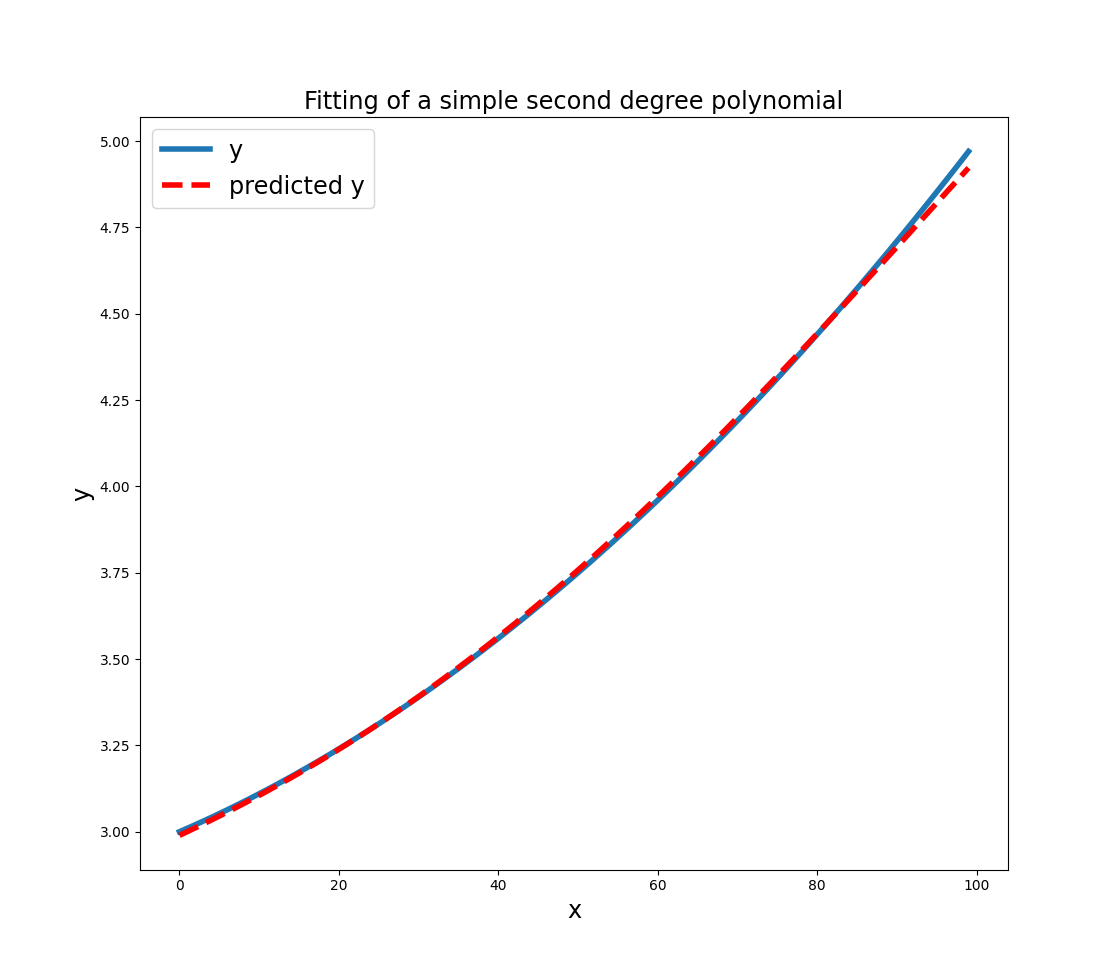
\includegraphics[width=5in]{figure/verification.png}}
\caption{Simple verification case}
\label{verification}
\end{figure}

\subsection{Datasets}

Below is a short description of each dataset used in this report, along with a table (Table.~\ref{datasettable}) listing their characteristics.

\subsubsection{Franke Function}

The Franke Function is a simple weighted sum of exponentials, taking two inputs and returning a real value. It is commonly used to test machine learning algorithms for regression problems. For our linear regression problems, our training data will be based on a 9th degree polynomial fit of the Franke Function, with 56 features. For the feed forward neural network, we will use the x and y values directly. The Franke Function is defined as follows.


\begin{multline}
f(x,y) = \frac{3}{4}e^{\left(-\frac{(9x-2)^2}{4}-\frac{(9y-2)^2}{4}\right)} +  \frac{3}{4}e^{\left(-\frac{(9x+1)^2}{49}-\frac{(9y+1)}{10}\right)} +
\frac{1}{2}e^{\left(-\frac{(9x-7)^2}{4}-\frac{(9y-3)^2}{4}\right)} - 
\frac{1}{5}e^{\left(-(9x-4)^2-(9y-7)^2\right)}.
\end{multline}

In practice, we add a normally distributed noise $N(0,0.05)$ to this function.

\subsubsection{Wisconsin Breast Cancer Dataset}

This dataset contains 30 features describing important characteristics of tumors. The features are real numbers. Each instance has an associated class, indicating whether the tumor was benign or not. This leads to a binary classification problem.

\subsubsection{MNIST 8x8}

This dataset contains a preprocessed set of black and white images of hand drawn digits. The images are 8 by 8 pixels, leading to 64 features, where each feature is an integer in the range $[0-16]$ describing the intensity of the pixel at that position\footnote{in reality, this describes the number of "on" pixels in a 4x4 region in the original image}. Each image has an associated class, which is simply the digit depicted. This leads to a multiclass classification problem with 10 classes.

\begin{table}[h]
\caption{Characteristics of each dataset used in the report}
\begin{center}
\label{datasettable}
\begin{tabular}{| c | l | l | l |}
\hline
Dataset & Number of instances & Features & Type \\
\hline
Franke Function (raw data) & 400 & 2 & regression \\
Franke Function (polynomial features) & 400 & 56 & regression \\
Wisconsin Breast Cancer & 569 & 30 & binary classification \\
MNIST 8x8 & 1797 & 64 & multiclass classification (10 classes) \\
\hline
\end{tabular}
\end{center}
\end{table}

\section{Results}

\subsection{Different schedulers used with linear regression}

In order to study the attributes of the different scheduler methods we performed numerical linear regression using gradient descent on the Franke Function with 56 polynomial features. This simple problem will allow us to gain an intuition of how the different schedulers compare against eachother. 

From  Fig.~\ref{constant_v_momentum}, we can observe that adding momentum improves upon the solutions found by the constant scheduler when using full batch gradient descent, reaching an MSE of 0.180 for the test data. By adding a memory of the previous gradients, we gain speed in the direction where most gradients point, speeding up our descent. This allows us to obtain a lower MSE scores in fever epochs, when compared to the constant scheduler's MSE of 0.198.

\begin{figure}[H]
\centerline{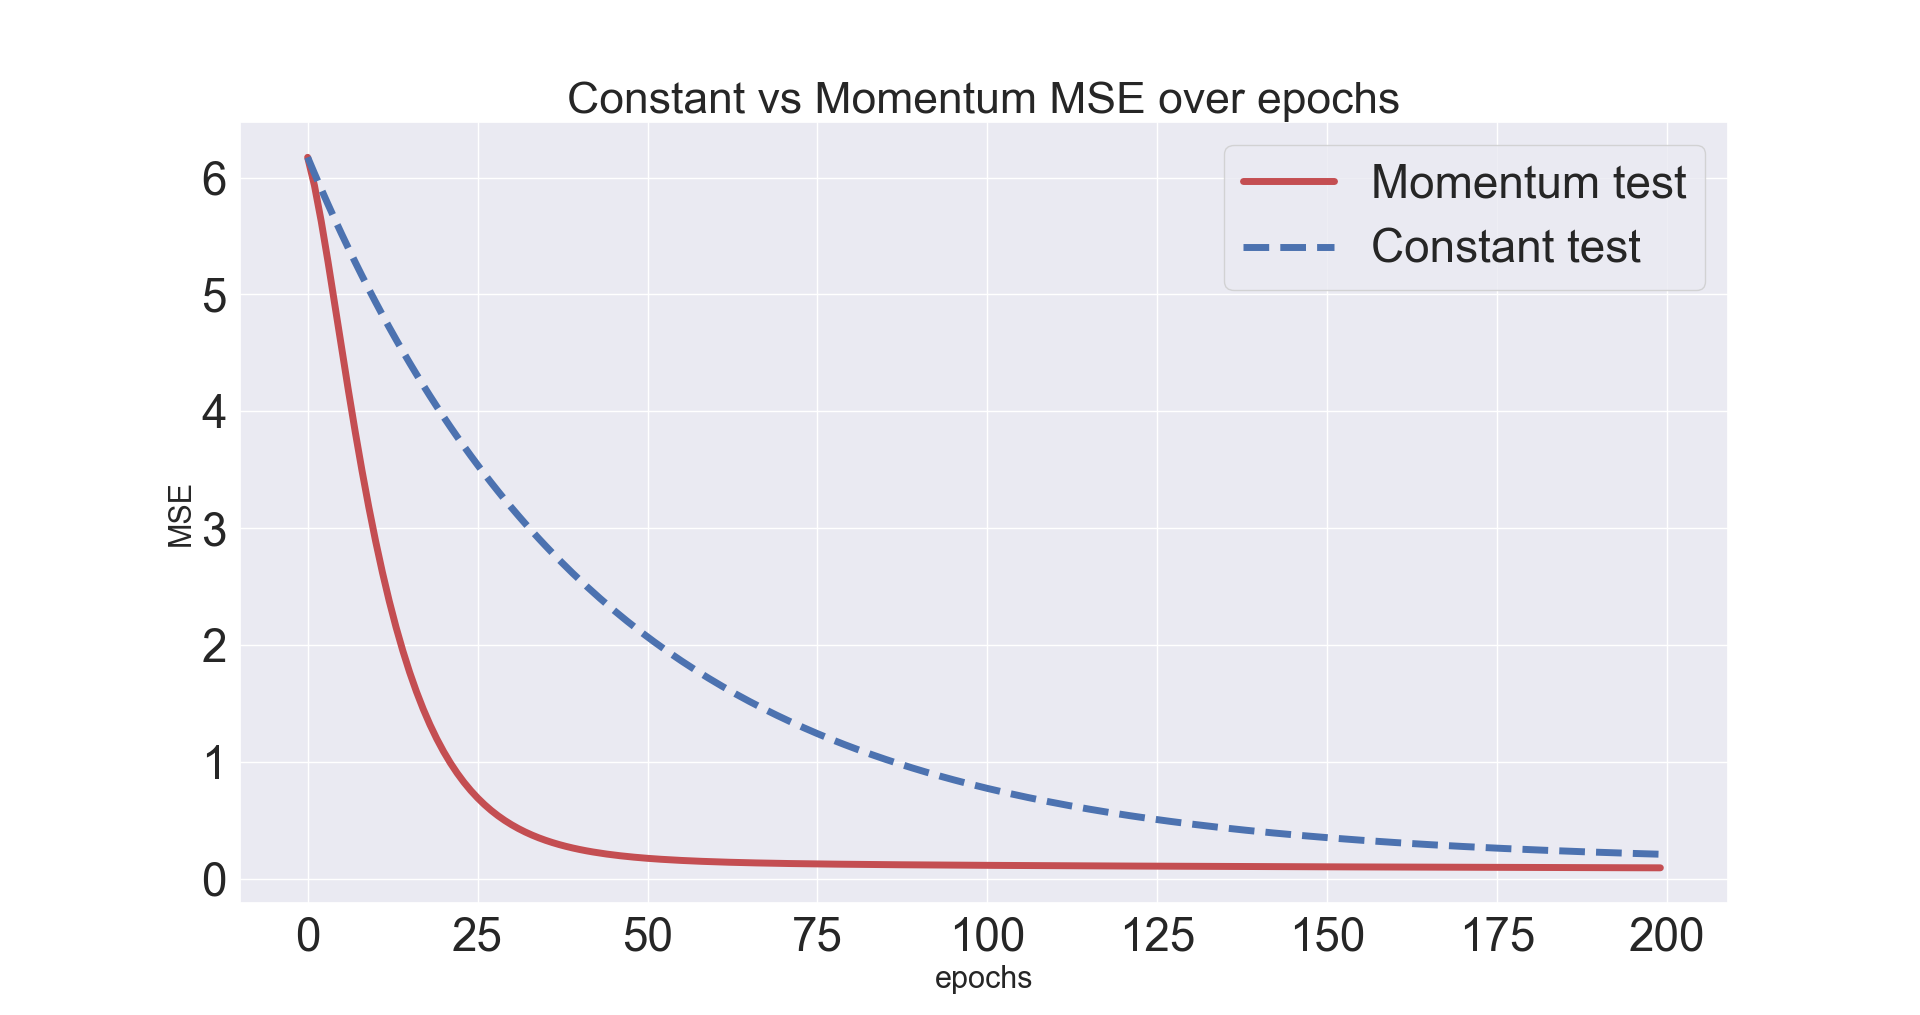
\includegraphics[width=5in]{figure/constant_v_momentum.png}}
\caption{Constant vs momentum MSE for test data plotted for 200 epochs using full batch gradient descent. The final MSE for Constant was 0.198, ten percent higher than Momentum's 0.180.}
\label{constant_v_momentum}
\end{figure}

By introducing mini-batch gradient descent, we can observe how decreasing the batch size improves our performance further (Fig.~\ref{batch_constant_v_momentum}). Mini-batch gradient descent clearly yields a lower MSE for the test data than full batch gradient descent for the same amount of epochs. The best result for both constant and momentum were reached for a batch size equal to 2, close to a fully stochastic gradient descent. The test data MSE reached $0.044$, an impressive improvement over constant's previous result of $0.198$ MSE with full batch gradient descent. Because we first gridsearched the optimal values of eta and lambda first with a predefined base batch size, we must acknowledge that these results will have some bias towards the batch size used when searching for the optimal hyperparameters. However, given that we have gridsearched with different base batch sizes accross our testing, we have found the results to be similar accross different base batch sizes, and that this bias which we induced to save computational time was insignificant. A full comparison of MSE over batch sizes for all the different schedulers can be viewed in Figure ~\ref{sgdbatch} in the appendix, where we can see that all schedulers yield increasingly better results as the batch size decreases.

\begin{figure}[H]
\centerline{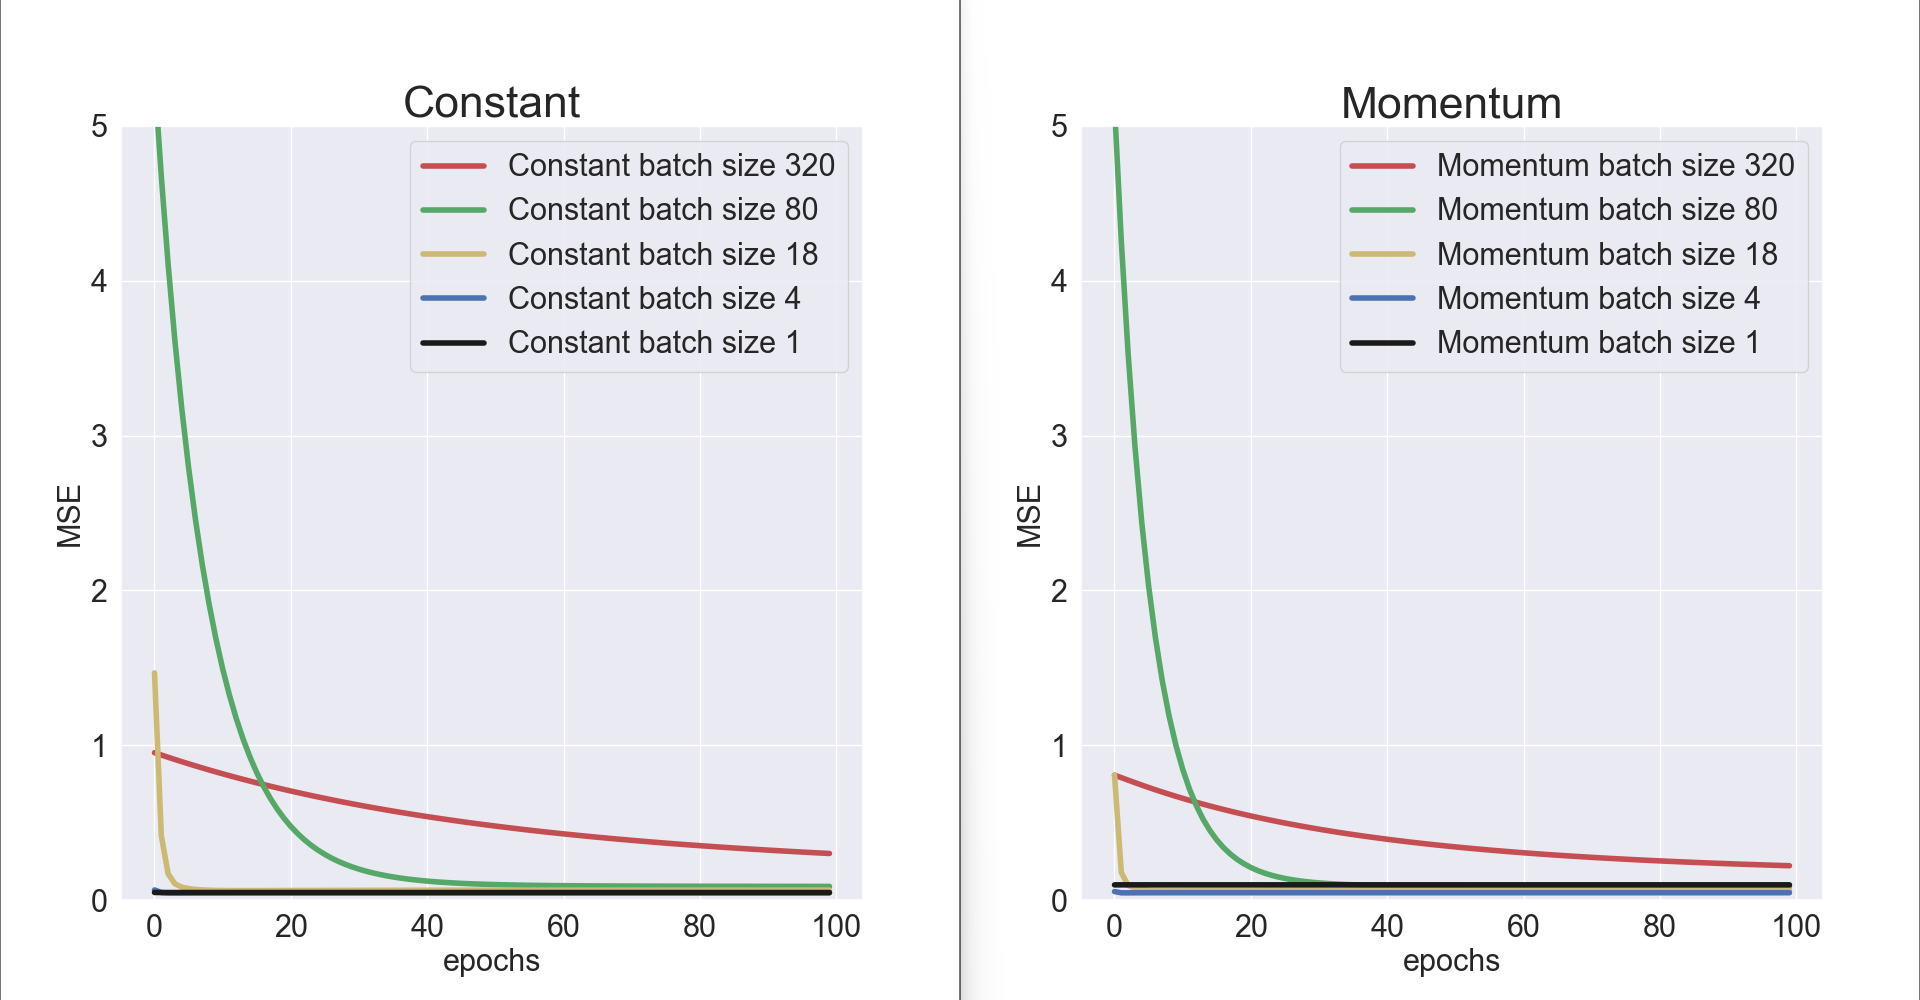
\includegraphics[width=6in]{figure/new_SGD_batch_momentum_constant.png}}
\caption{Constant vs momentum test MSE for different batch sizes, plotted for 200 epochs using full batch gradient descent. A batch size of 320 is full batch GD, whilst a batch size of 1 is fully stochastic GD.}
\label{batch_constant_v_momentum}
\end{figure}

Furthermore, with the introduction of various adaptive scheduler methods such as RMS prop, Adagrad (with and without momentum) and adam we can observe from Fig.~\ref{figall} that we can reach even greater results in fewer epochs. In order to get a better understanding of the computational cost we have also compared the time it took to fit the data to an MSE of 0.200. Looking at Table.~\ref{timetable}, Adagrad took the least time, reaching the target MSE almost 50 times faster our constant scheduler. Based on Fig.~\ref{figall}, Adam seems to reach an MSE of 0.2 the fastest when strictly looking at the number of epochs required. However, whilst Adagrad requires more epochs the computations are computed faster in our implementation. Surprisingly, RMS prop performed more poorly than expected compared to other adaptive schedulers.

\begin{figure}[H]
\centerline{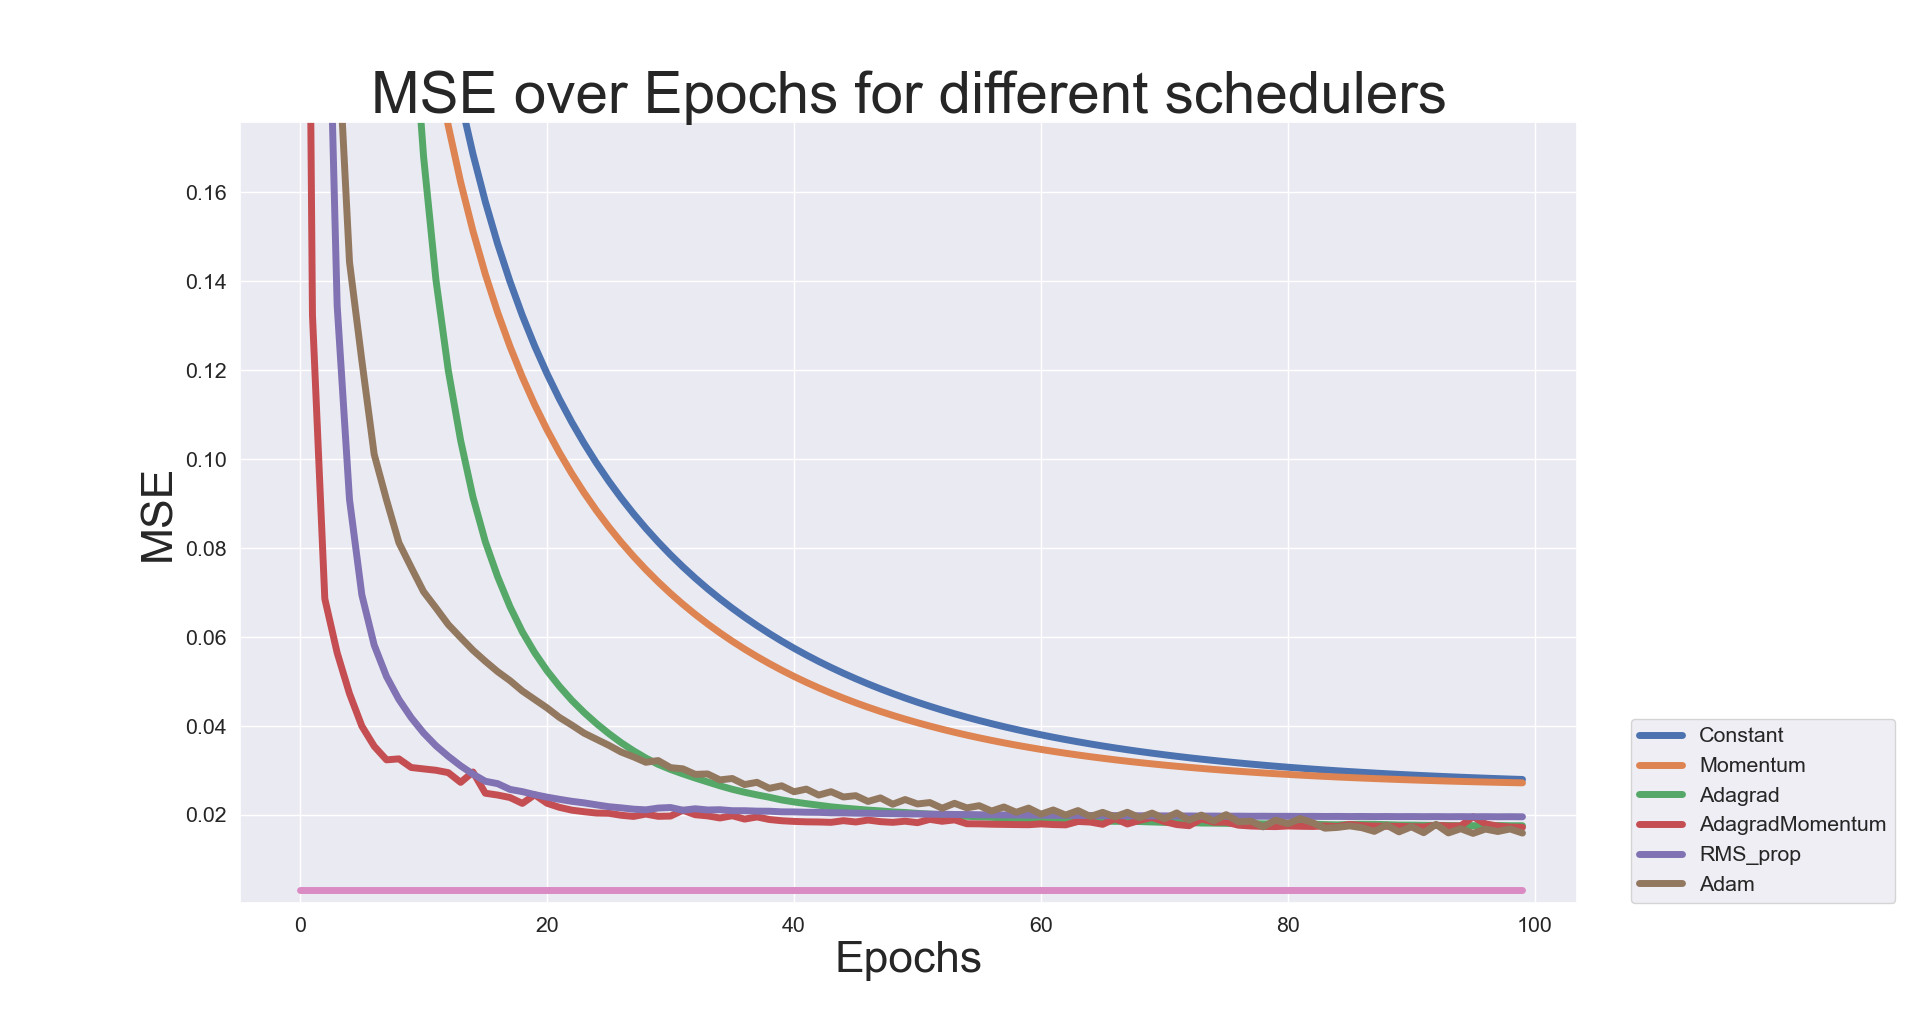
\includegraphics[width=7in]{figure/new_adam_v_adagrad.png}}
\caption{Test MSE over epochs for all schedulers}
\label{figall}
\end{figure}

\begin{table}[H]
\caption{Table over time take for each scheduler}
\begin{center}
\label{timetable}
\begin{tabular}{| c | l |}
\hline
Scheduler & Time to reach 0.2 test MSE \\
\hline
Constant & 0.601 \\
Momentum & 0.513 \\
RMS\_prop & 0.330 \\
AdaGrad & 0.013 \\
AdaGrad with Momentum & 0.014 \\
Adam & 0.041 \\
\hline
\end{tabular}
\end{center}
\end{table}

An interesting insight from Fig.~\ref{heatmap} is that all the schedulers prefer high learning rates and regularization. As this plot was generated for 100 epochs due to the computational complexity of gridsearching the six schedulers, the bias towards higher learning rates is certainly due to the high learning rates being able to reach a low MSE in the short training time. With the lambda = 0 column representing the ordinary least squares solutions, these are clearly consistantly outperformed by Ridge regression as the best MSE is achieved with regularization. We can see that the addition of a momentum term makes a small difference for both the constant scheduler, as well as with Adagrad. However, we can see that adaptively changing the learning rate, like Adagrad, RMS prop and Adam does, has a much bigger impact on the final MSE than the momentum term.

\begin{figure}[H]
\centerline{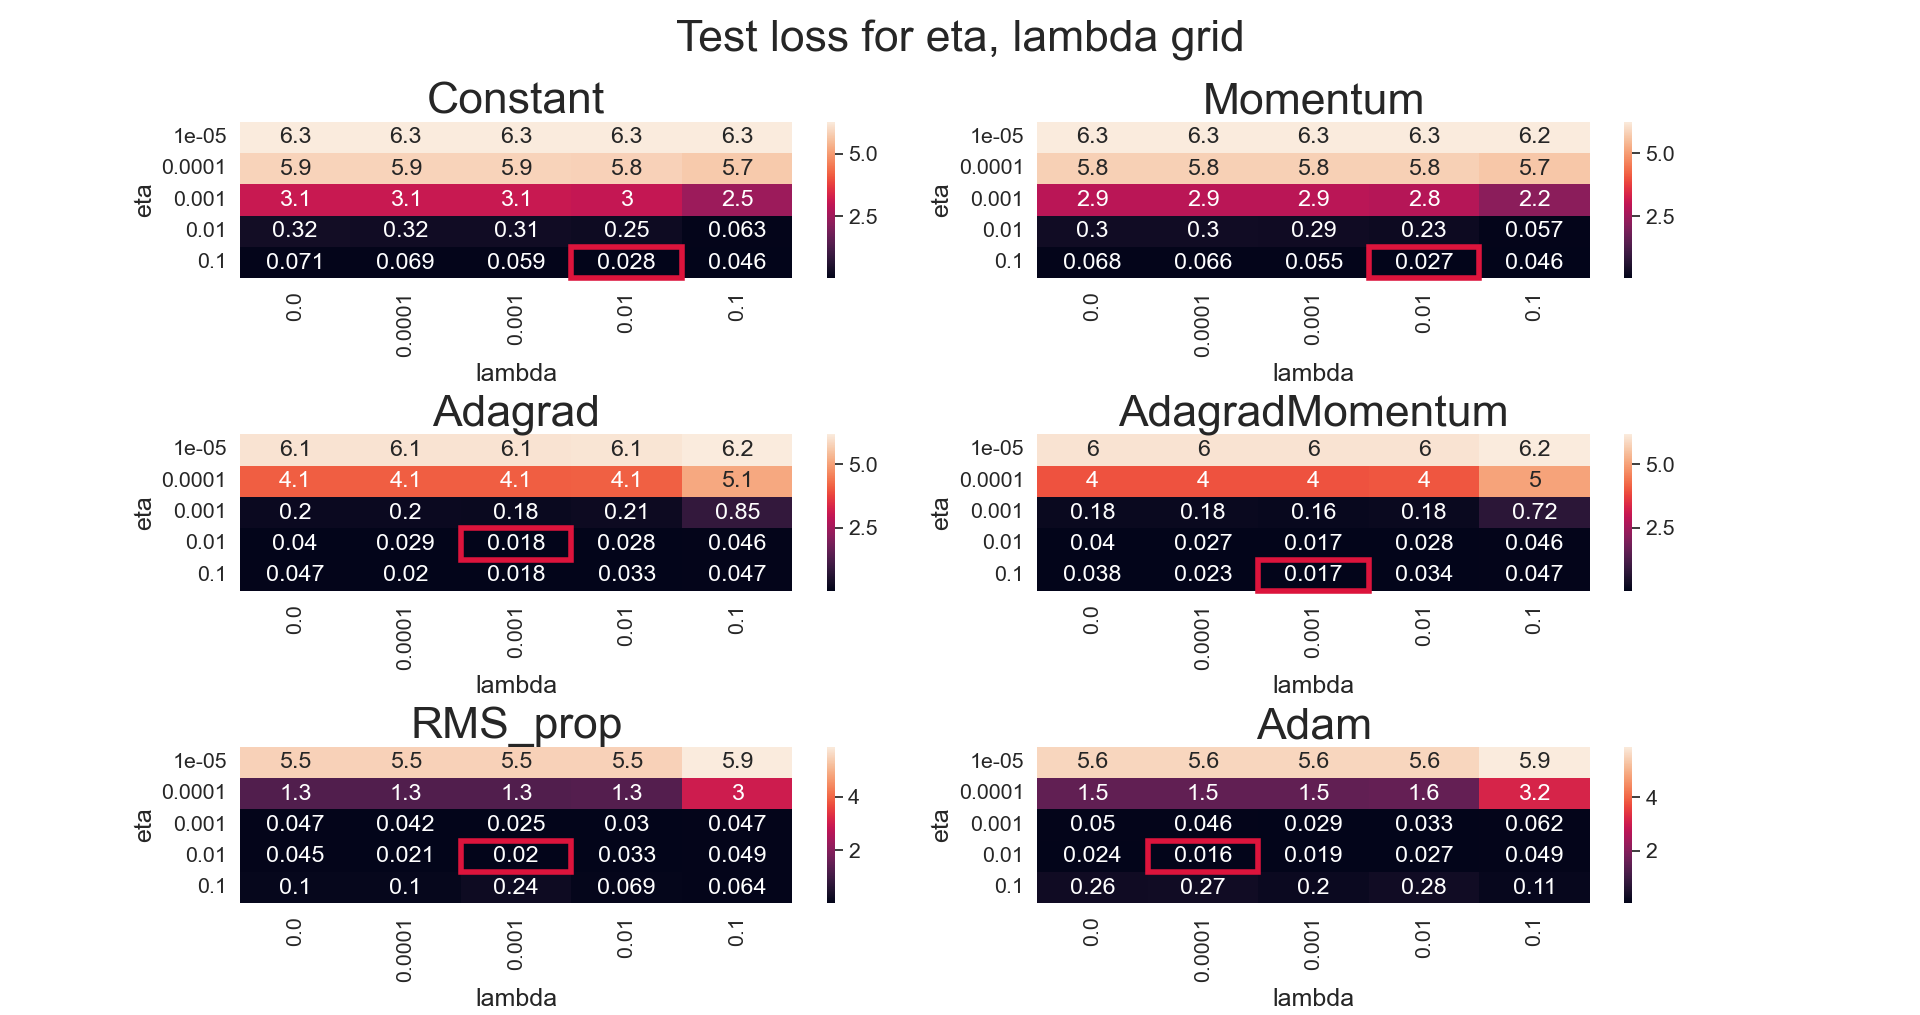
\includegraphics[width=8in]{figure/new_100e_gridsearch.png}}
\caption{MSE score gridsearch for hyperparameters eta, lambda for different schedulers}
\label{heatmap}
\end{figure}

Based on these findings, we decided to push Adagrad and Adam further, allowing them to run for much longer. After 5000 epochs, we reached an MSE of $0.012$ for Adam and $0.011$ for Adagrad. The plot for the MSE over epochs can be found in the appendix (Fig.~\ref{adam_v_adagrad}).


%100 epochs are more or less the same. As the largest change in MSE occurs in the first 50 epochs as seen in Fig.~\ref{figall}, perhaps the other schedulers are given enough time to catch up as the best performing schedulers, such as Adagrad, starts slowing down the rate at which the MSE is decreased. However, as can be seen in Fig.~\ref{heatmap}, Adagrad offers a 12\% \footnote{$\frac{constant MSE}{adagrad MSE} * 100 = \frac{0.018}{0.015} * 100 = 12\%$} decrease in MSE compared to the constant scheduler. It is clear from the results thus far that Adagrad is the best scheduler for approximating the Franke function when using linear regression with gradient descent. We believe that the reason Adagrad wins out is that these result are based on training for 100 epochs. The downfall of Adagrad in the literature seems to be that the aggressive decaying of the learning rate hinders a quick convergence deeper into training \cite{datasci}. We are thus cautionary to claim that Adagrad will do the best job over a much larger amount of epochs when compared to adaptive schedulers that claim to improve this aspect such as Adam.

% To test this, we compared Adagrad with Adam over 5000 epochs, cross validated for 5 folds, as can be seen in Fig.~\ref{adam_v_adagrad}. Both schedulers perform almost equally, with Adagrad reaching a slightly lower MSE of 0.011 for the test data when compared to Adam's 0.012. It could be argued that 5000 epochs is not enough for the improvements of Adam to be noticeable, as the MSE could still be pushed much lower. However, for these computationally expensive runs it is clear that Adagrad is the scheduler of choice, especially considering our previous conclusion that Adagrad used less time to train. It should be noted that scikit learn's implementation outperforms both our implementation of Adagrad and Adam, with an MSE of 0.004. This could be due to a more favorable wight initialization in scikits model, along with additional optimizations implemented in their library. That we don't beat the analytical solution is no surprise, as we have limited ourself to a polynomial approximation of the Franke Function with 56 features. Our MSE might approach the analytical MSE, but this might take an unreasonable amount of epochs considering the computational runtime. Still, we have obtained an MSE lower than the Newton method's result of 0.020, even though it was at a much greater computation. Next, we investigate the use of linear regression in a neural network with hidden nodes, such that we can free ourselves of the limitations of the polynomial approximation.


\subsection{Neural Network for regression}

Having gained an understanding of how the different schedulers function, and having created the necessary infrastructure to study our models' performance based on a number of different factors, we use these methods to optimize our neural network for linear regression. More specifically, we attempt to fit the Franke function. First, we perform a preliminary test on MSE over model complexity. For comparisons sake, we use the same scheduler for each architecture, and fix the regularization parameter at 0. By fixing the regularization parameter at 0, we are of course favouring less complex models, but this a good way to get a general sense of when the model starts to overfit. Using the sigmoid activation function, we can study the MSE as a function of the total hidden node count (Fig.~\ref{msebymodelfranke}). Here we see, somewhat surprisingly, that our train and test MSE are not deviating particularly much from eachother, even with very complex networks. There are many reasons that this may be the case. As we have stated before, once we start using numerical methods, computational effort becomes a large factor in any test one does, and many decisions have to made regarding how much time can be spent on each test. Due to these computational constraints, we have not been able to grid search for the best parameters for each model complexity, nor have we been able to train for more than 200 epochs for each model. These shortcomings will greatly affect how our models perform, as it is unlikely that each model uses the same learning rate and scheduler, or that more complex models use the same amount of epochs to train their weights. Based on this, we can assume that the higher complexity models have not been trained enough, and that this explains why both their train and test MSE are higher than the less complex models. Regardless, it seems that for up to about 200 total nodes, three hidden layers does the best, and as such we chose an architecture of three hidden layers with 66 nodes each (which is where we achieved our lowest MSE).

\begin{figure}[H]
\centerline{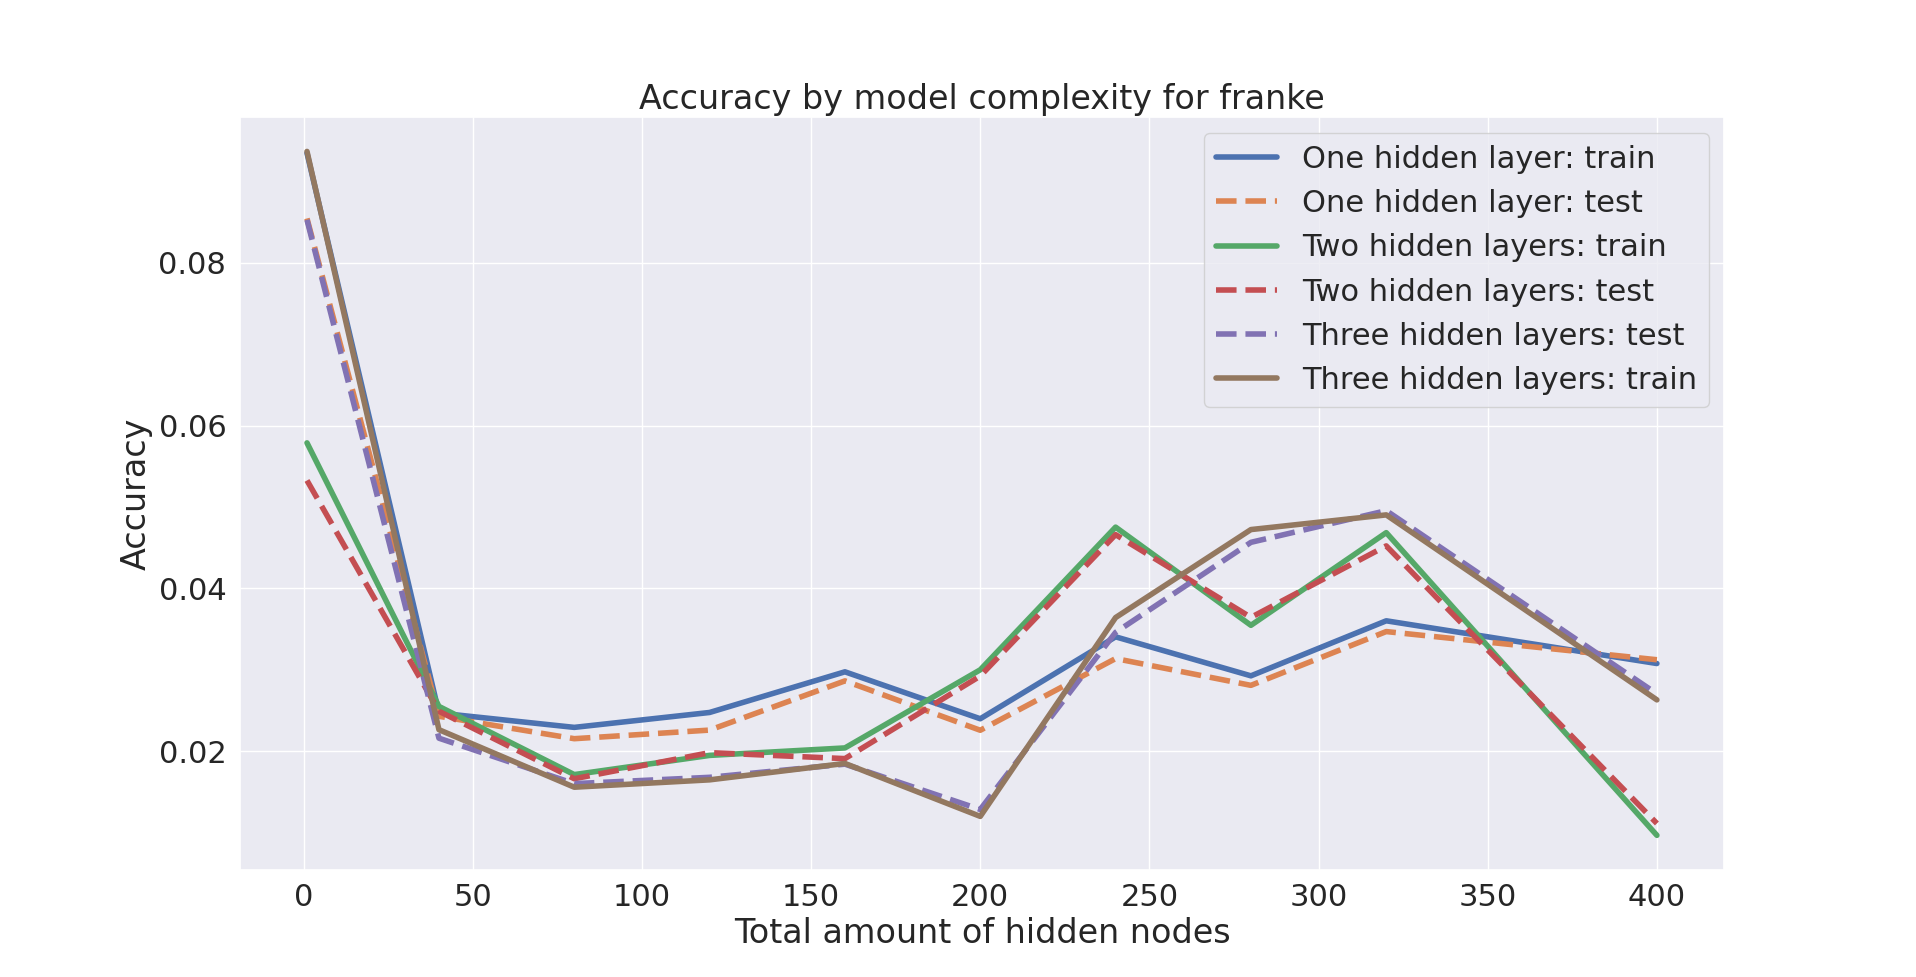
\includegraphics[width=6in]{figure/msebymodelfranke.png}}
\caption{Comparison between a neural net with one hidden layer, and one with two hidden layers, for different totals of hidden nodes. For the network with two hidden layers, the total is evenly divided between the layers, such that at $x = 60$ we have a network with two hidden layers of 30 nodes each. In this case, the hidden layers used the sigmoid activation function.}
\label{msebymodelfranke}
\end{figure}

Using this architecture, we performed a gridsearch. Due to time constraints, we have felt it necessary to limit our gridsearch to only two schedulers. Based on our testing with linear regression with gradient descent, we have seen that Adam and Adagrad seems to be the best performers. Based on Goodfellows recommendations, we started with the RELU activation function \cite[188]{gbc}. With this, we found Adam to be the best scheduler, with an eta of 0.01 and no regularization. However, when using these parameters, we encountered the so called "dying RELU problem", where too many of our RELU nodes output zero, leading to our gradient descent slowing down and eventually stopping completely. A better weight initialization, for example using Xavier Initilization, could solve this problem, but another way to circumvent this issue is to use Leaky RELU. This activation function has a small but non-zero gradient for negative values, instead of zero as with RELU. Gridsearching with Leaky RELU instead gave the exact same parameters.

Using these parameters along with Adam and LRELU, we acheived an MSE of $0.004781$, which is better than the results gained using gradient descent on our polynomial fit. We can see that by not forcing our model to try and find a polynomial fit, we are achieving better results. However, we are still not able to beat the analytical solution to the best polynomial fit at polynomial degree 9, which is somewhat disappointing. A possible explanation for this is that the Franke function can be represented as a weighted sum of polynomials, and as such a polynomial fit is especially suited to approximate this function. Our neural net must learn the relation between the inputs and outputs on its own, a process which is computationally intensive and difficult. Looking at our predicted terrain (Fig.~\ref{predterrain}), we can see that our prediction is somewhat reasonable, but not entirely convincing. Furthermore, we can see that the polynomial fit seems to match the actual terrain more closely, which it achieves in a fraction of the runtime.

\begin{figure}[H]
\centerline{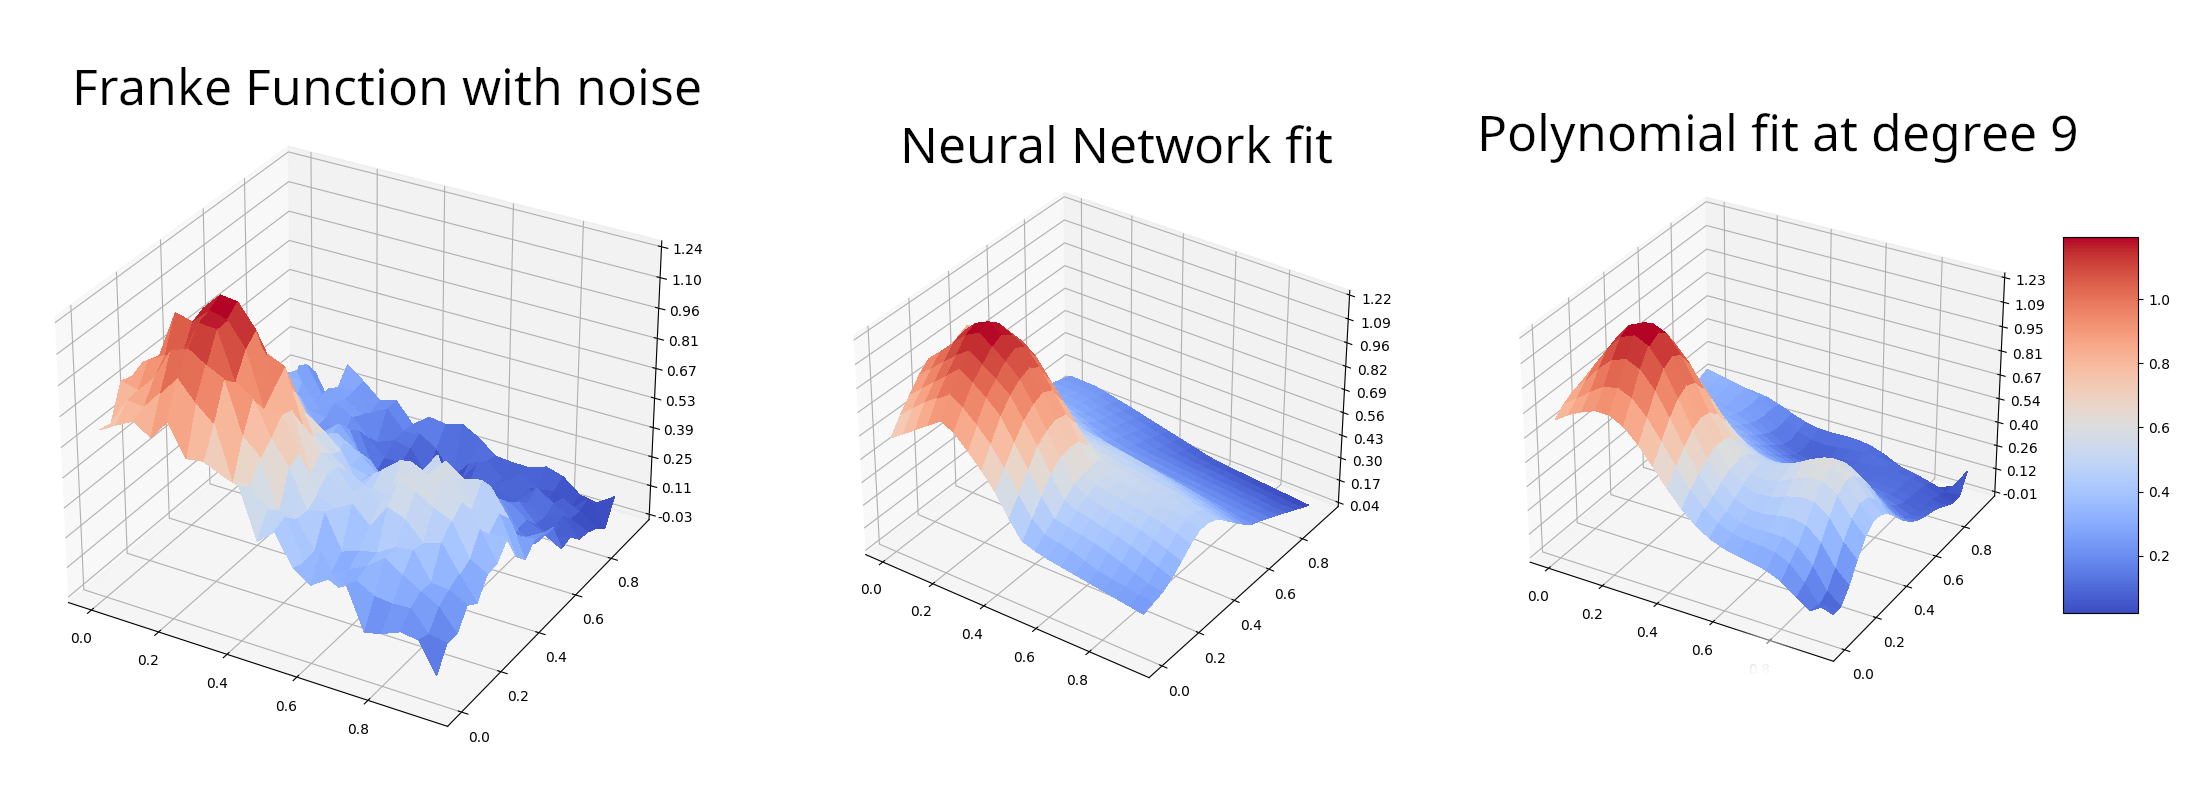
\includegraphics[width=7in]{figure/Franke_fit_66x3_lam0.png}}
\caption{Surface plot of the actual terrain created by the Franke function, the best fit achieved by our Neural Network, and the best polynomial fit for polynomial degree 9}
\label{predterrain}
\end{figure}

\subsection{Neural Network for binary and multiclass classification}

With mediocre results on regression, we turn to classification. To test our neural networks ability to solve classification problems, we first applied it to the Wisconsin Breast Cancer dataset. But to get the best results, there are a large amount of parameters that need to be decided on. We must find the best architecture, the best activation functions, the best scheduler and the best parameters for said scheduler. Finding the absolute best combination of all these choices is impossible, so compromises must be made.

We start by trying to find a good model complexity, i.e the best number of hidden layers, and the amount of nodes in them. To do this, we plotted the accuracy over different model architectures. Like we did during regression, we fix all the other parameters and study the architecture by itself. Using the sigmoid activation function (Fig.~\ref{cancerarchcompsigmoid}), our results are somewhat surprising. We see that even at 400 total hidden nodes, we are not overfitting. This implies that the dataset is quite homogenous, and that the test set is very similar to our training set. With such a dataset, it is possible to gain a very good fit using more and more complex models, although the computational effort obviously increases as well. Moreover, it is not given that instances outside this dataset are as homogenous as the relatively small (569) sample we have here, so one should be careful to use an overcomplex model even if it does not hurt the test accuracy for this particular dataset. Using the RELU activation function, the results are quite different, as can be seen in Fig.~\ref{cancerarchcomp}. Here we can observe that a neural net with two or three hidden layers starts performing very inconsistently when the number of nodes increases. Looking more closely at the training process, we can see that training stops completely in some of our crossvalidations. Clearly, we are again running into the "dying RELU problem". Here we can clearly see some of the benefits of the sigmoid, as even if the gradients become very small, they will never be zero, as with RELU. Regardless, we see similar performance for RELU using only one hidden layer. Based on these findings, we decided to use a model with a single hidden layer of 100 nodes, using the RELU activation function.

\begin{figure}[H]
\centerline{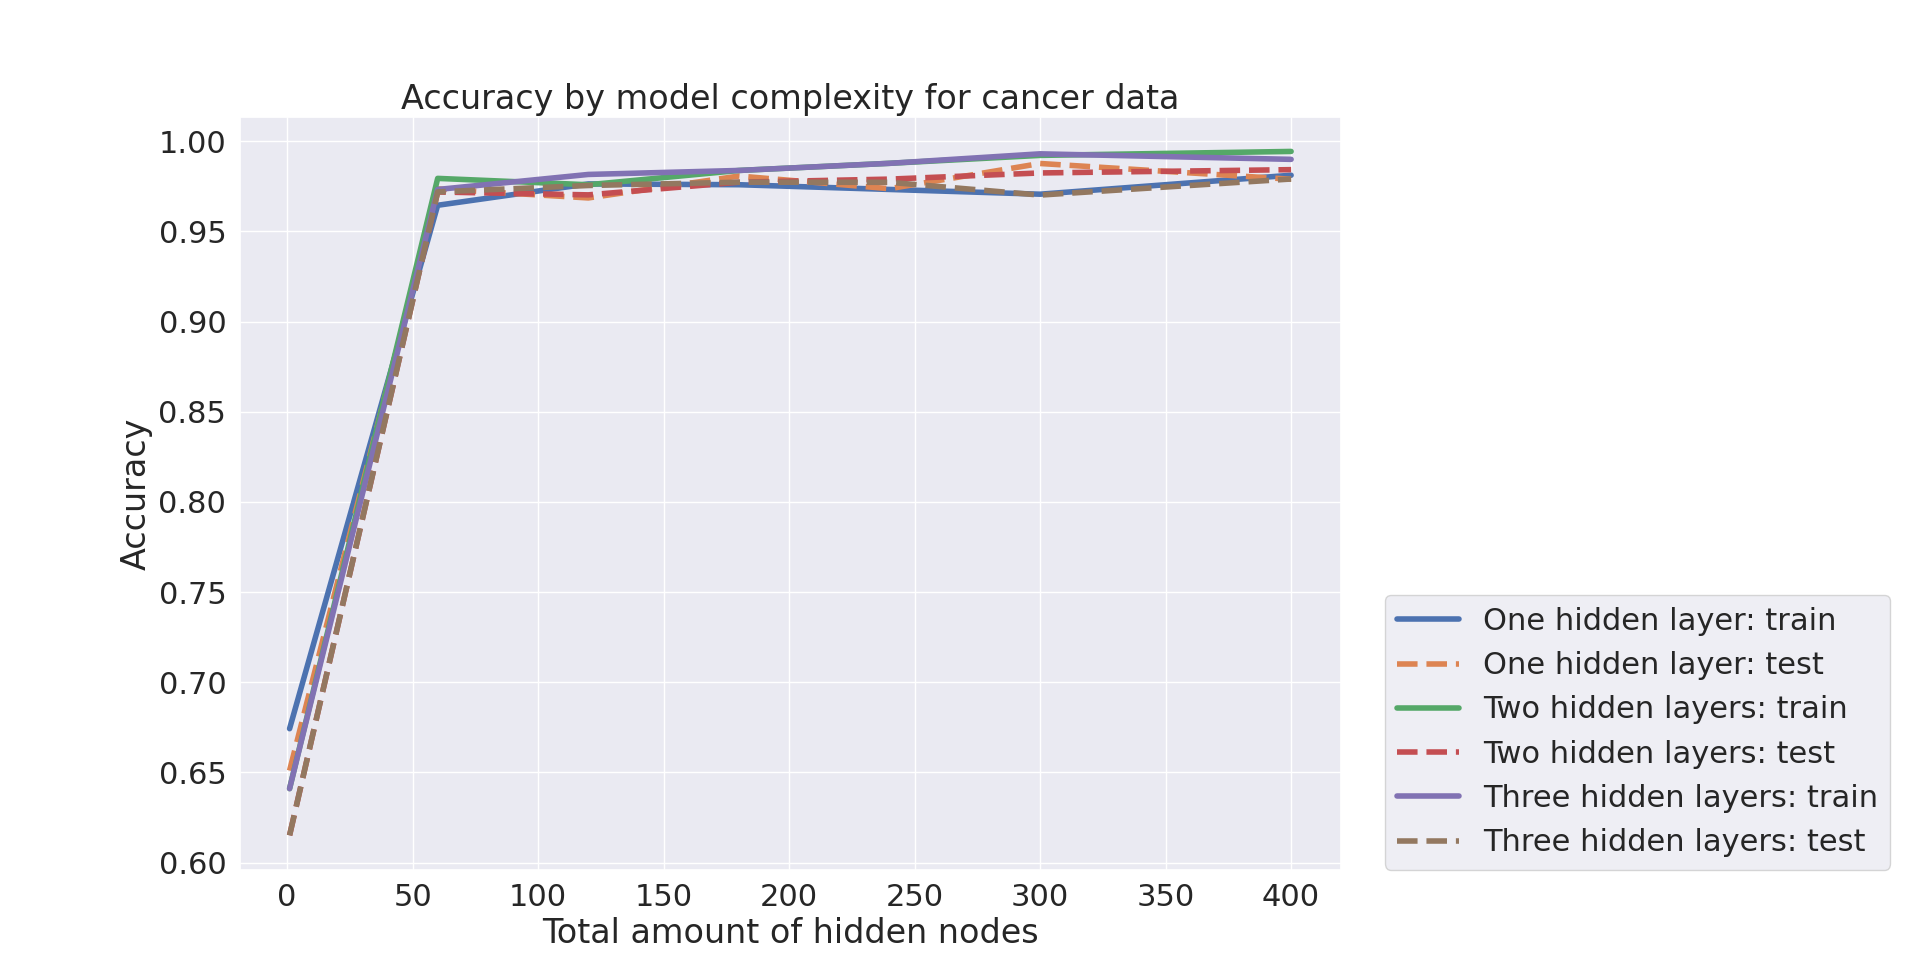
\includegraphics[width=6in]{figure/cancerarchcompsigmoid.png}}
\caption{Comparison between a neural net with one hidden layer, and one with two hidden layers, for different totals of hidden nodes. For the network with two hidden layers, the total is evenly divided between the layers, such that at $x = 60$ we have a network with two hidden layers of 30 nodes each. In this case, the hidden layers used the sigmoid activation function.}
\label{cancerarchcompsigmoid}
\end{figure}

\begin{figure}[H]
\centerline{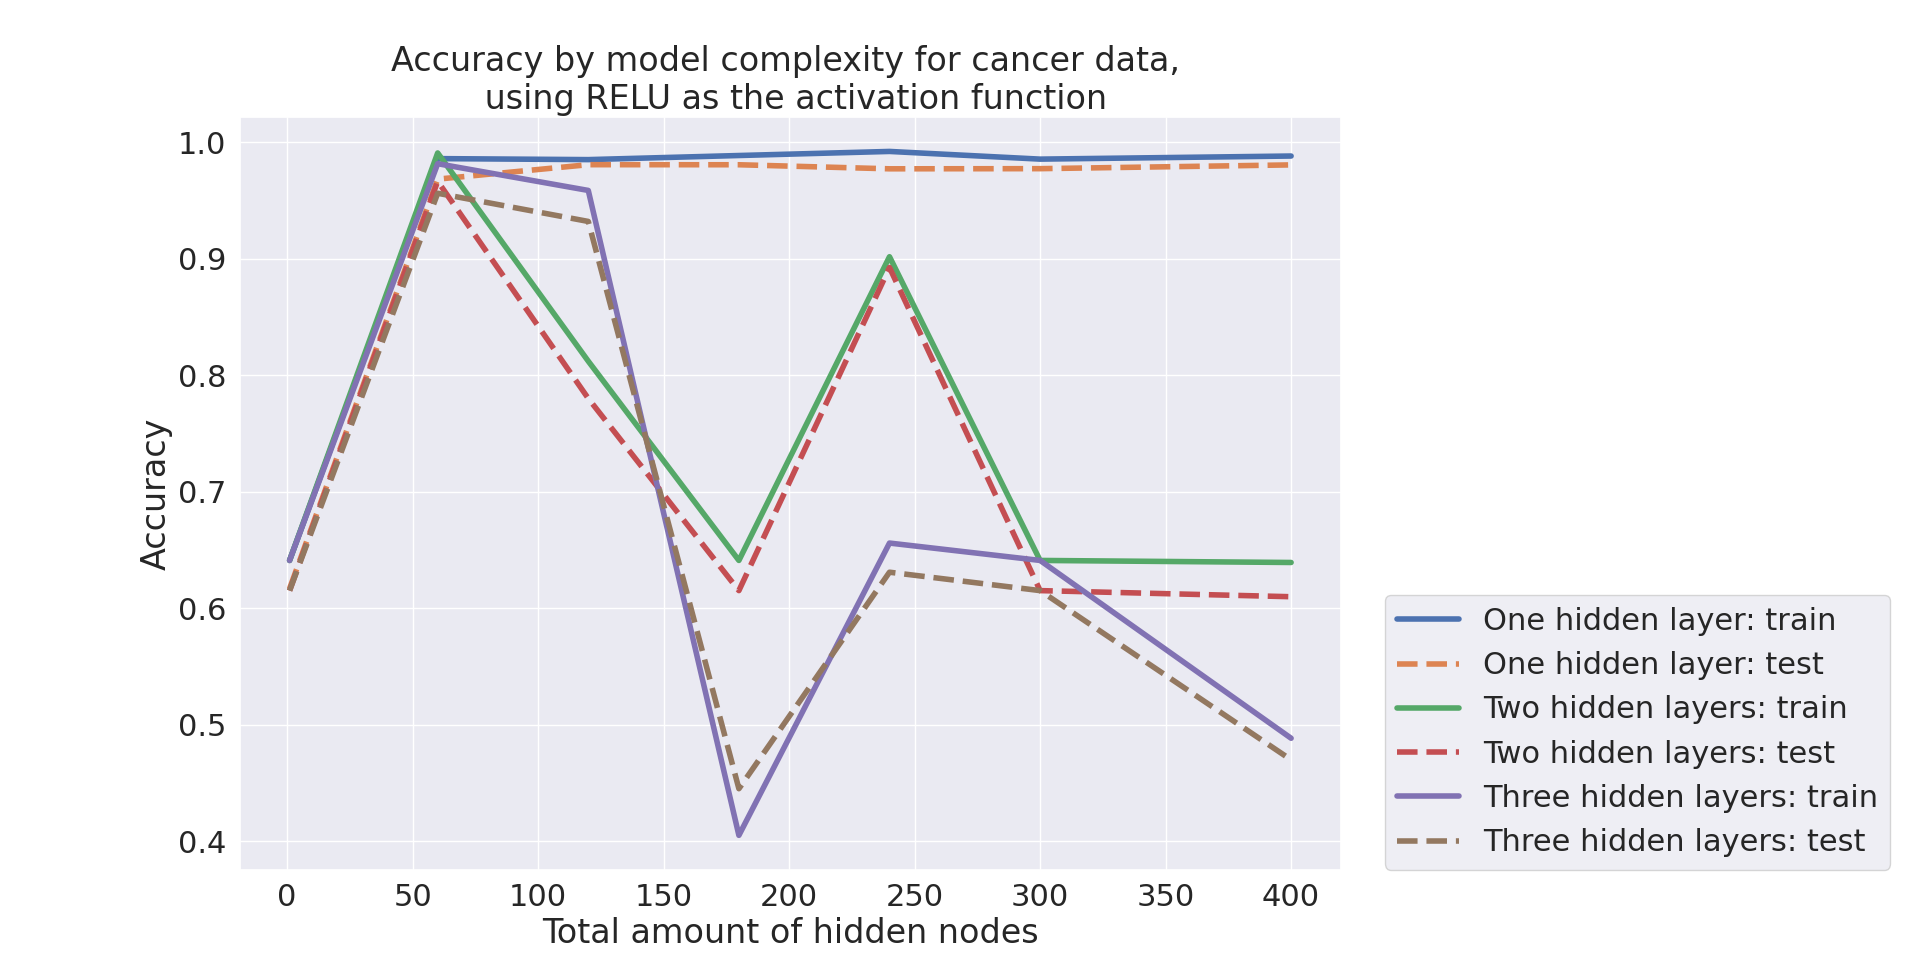
\includegraphics[width=6in]{figure/cancerarchcomp.png}}
\caption{Comparison between a neural net with one hidden layer, and one with two hidden layers, for different totals of hidden nodes. For the network with two hidden layers, the total is evenly divided between the layers, such that at $x = 60$ we have a network with two hidden layers of 30 nodes each. In this case, the hidden layers used the RELU activation function.}
\label{cancerarchcomp}
\end{figure}

Using our gridsearch method on this model, we found that the best scheduler was Adam, with an eta of $0.001$ and a lambda of $0.0001$. With this combination of architecture and scheduler, we were able to achieve a crossvalidated test accuracy of $98.59\%$, which is a great result. This outperforms SciKit's MLP classifier, which achieved a crossvalidated test accuracy of around $95\%$. Looking at the confusion matrix (Fig.~\ref{cancerconf}), we see that we are achieving good predictions for both true positives and true negatives.

\begin{figure}[H]
\centerline{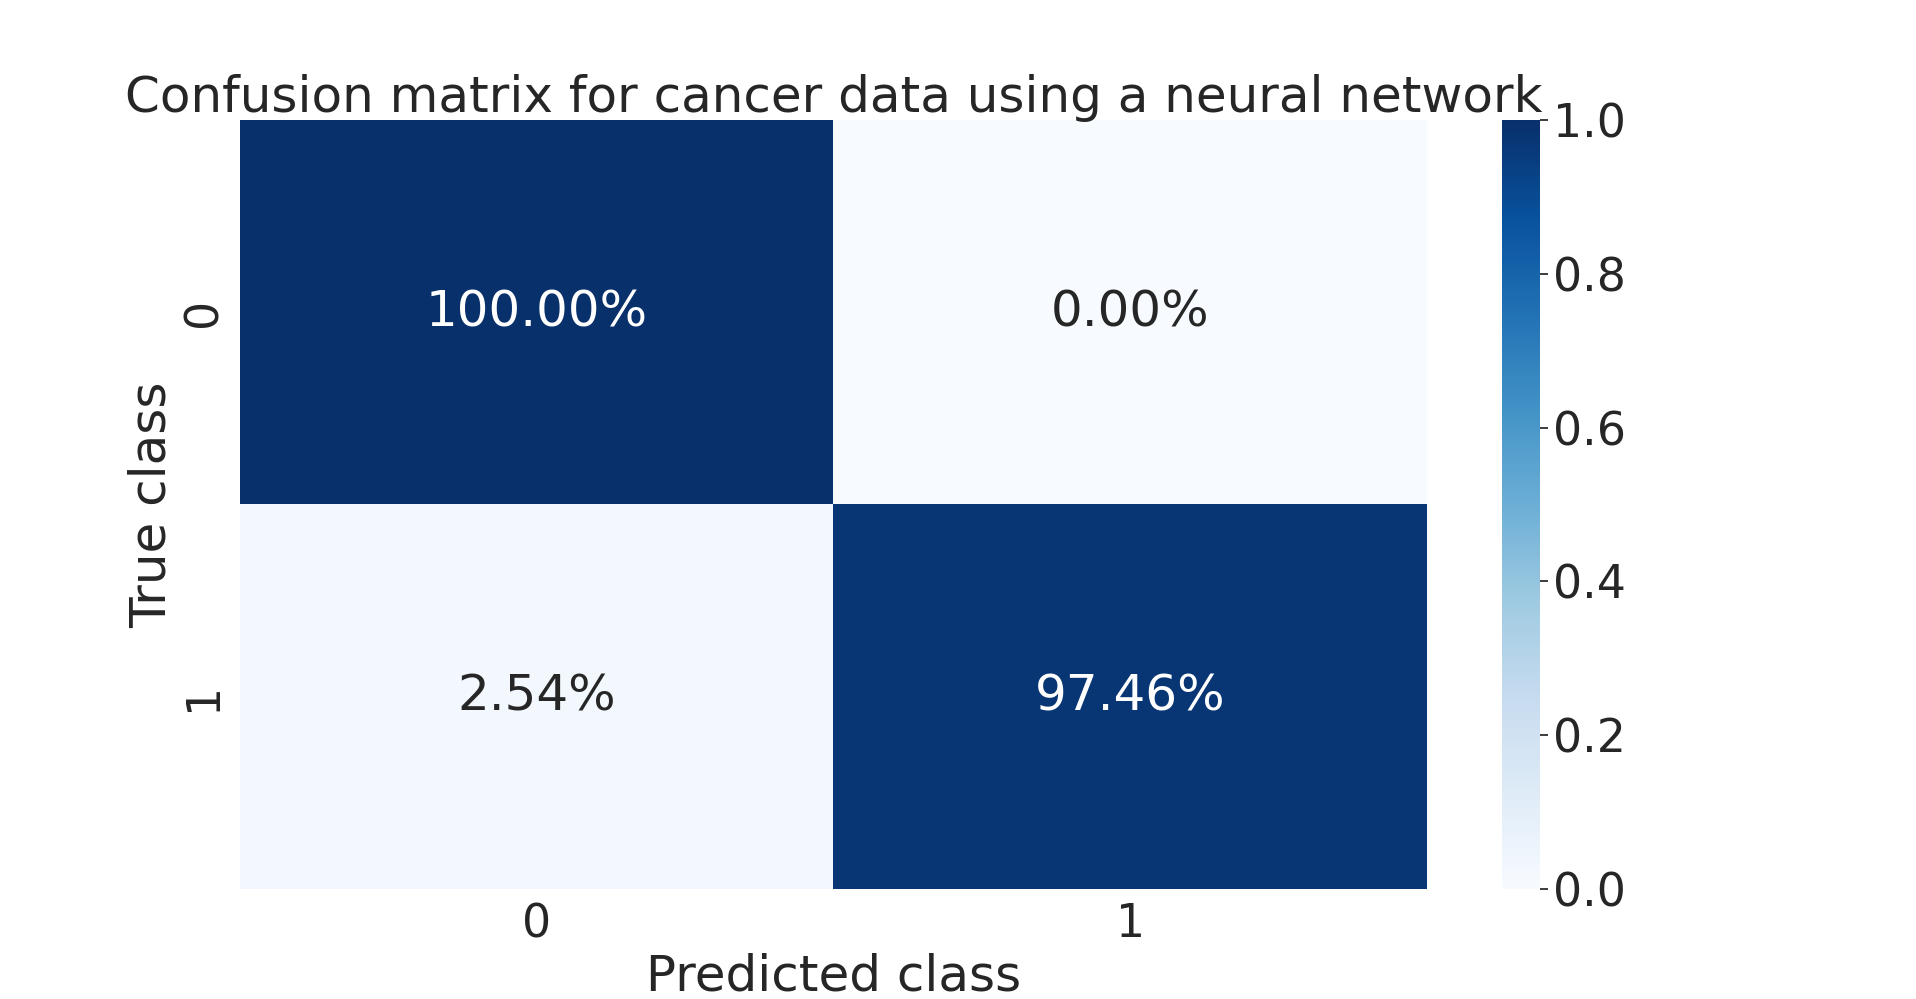
\includegraphics[width=5in]{figure/conf_mat_NN_cancer.png}}
\caption{Confusion matrix for the cancer dataset using a neural net with a single hidden layer of 60 nodes}
\label{cancerconf}
\end{figure}

Confident in our networks's ability to do binary classification, we turned to the MNIST dataset. Here, we perform an educated guess on the different parameters, based on our previous testing. We decided upon an architecture of a single layer with 100 nodes using the RELU activation function. For our scheduler, we used Adam with an eta of $0.001$ and no regularization. Being a multiclass problem with ten different classes, one might expect our neural network to struggle more with this dataset. However, this was not the case, as we achieved a crossvalidated test accuracy of $99.07\%$. Based on these results, we conclude that the initial guess for our model was a good one, and that further optimization has little room for improvement. From these two datasets, we can see that a neural network is adept at solving classification problems. On the other hand, these good results, and the ease with which our network attained them, could imply that the problems we have dealt with are not as complicated as they may seem.

\subsection{Logistic Regression}

Based on our good results with the neural net, we attempt to solve the same problems using simple logistic regression. Using logistic regression on the cancer dataset, we found through our gridsearch that Adam with an eta $0.1$ gave the best results. Here we found that logistic regression performed essentially equivalent to our neural net, achieving a test accuracy of $98.76\%$. Looking at Fig.~\ref{cancerlogneur}, we see that logistic regression keeps up and even surpasses our neural network in accuracy over epochs. The value of logistic regression becomes even greater when we consider the computational cost of each method. In this case, the logistic regression was about 65\% faster\footnote{The time taken to complete a crossvalidation with 5 folds up to 200 epochs was about 52 seconds for our neural network, but only 18 seconds for logistic regression}, with results surpassing our neural network (see Fig.~\ref{cancerconflog}). In the MNIST dataset, logistic regression also performed well, achieving an accuracy of $99.54\%$. This implies that our classification datasets were perhaps too simple, and that using Neural Networks was not needed to achieve good results. 
	
\begin{figure}[H]
\centerline{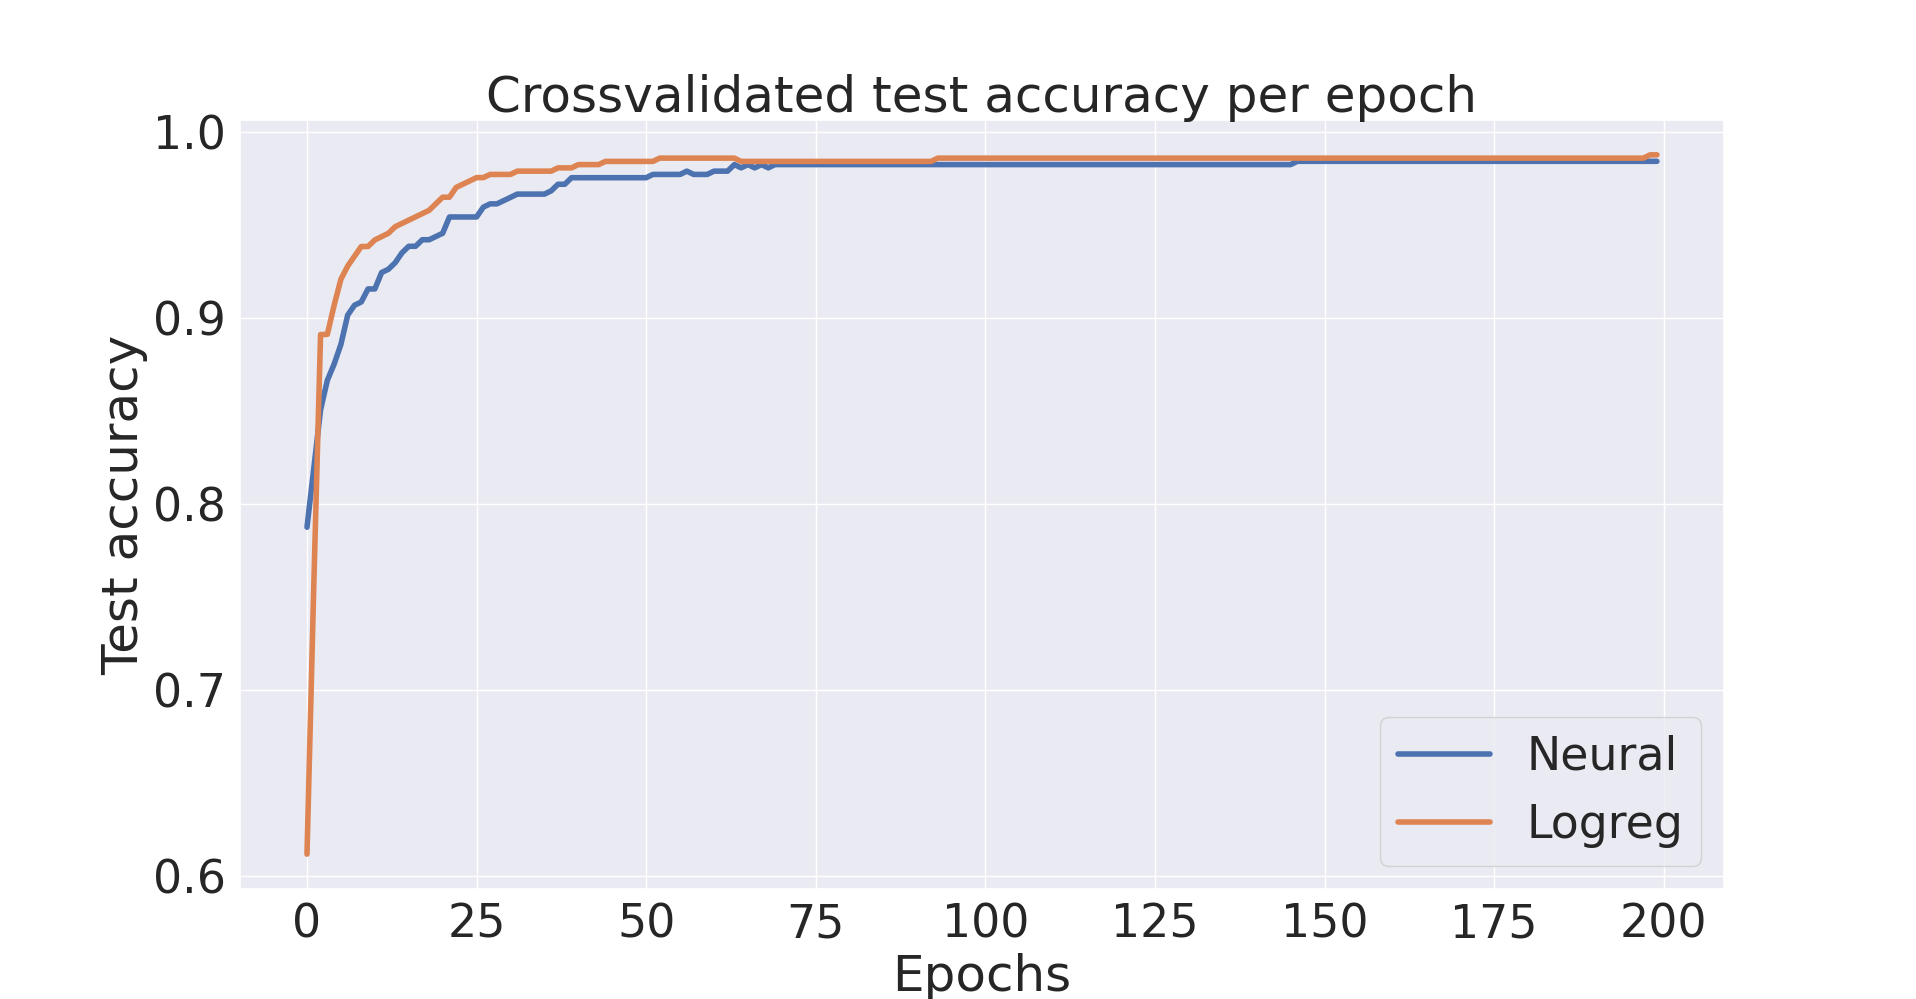
\includegraphics[width=5in]{figure/comp_NN_logreg_cancer.png}}
\caption{Comparison between the test accuracy of logistic regression and a neural network on classifying the cancer dataset}
\label{cancerlogneur}
\end{figure}
\begin{figure}[H]
\centerline{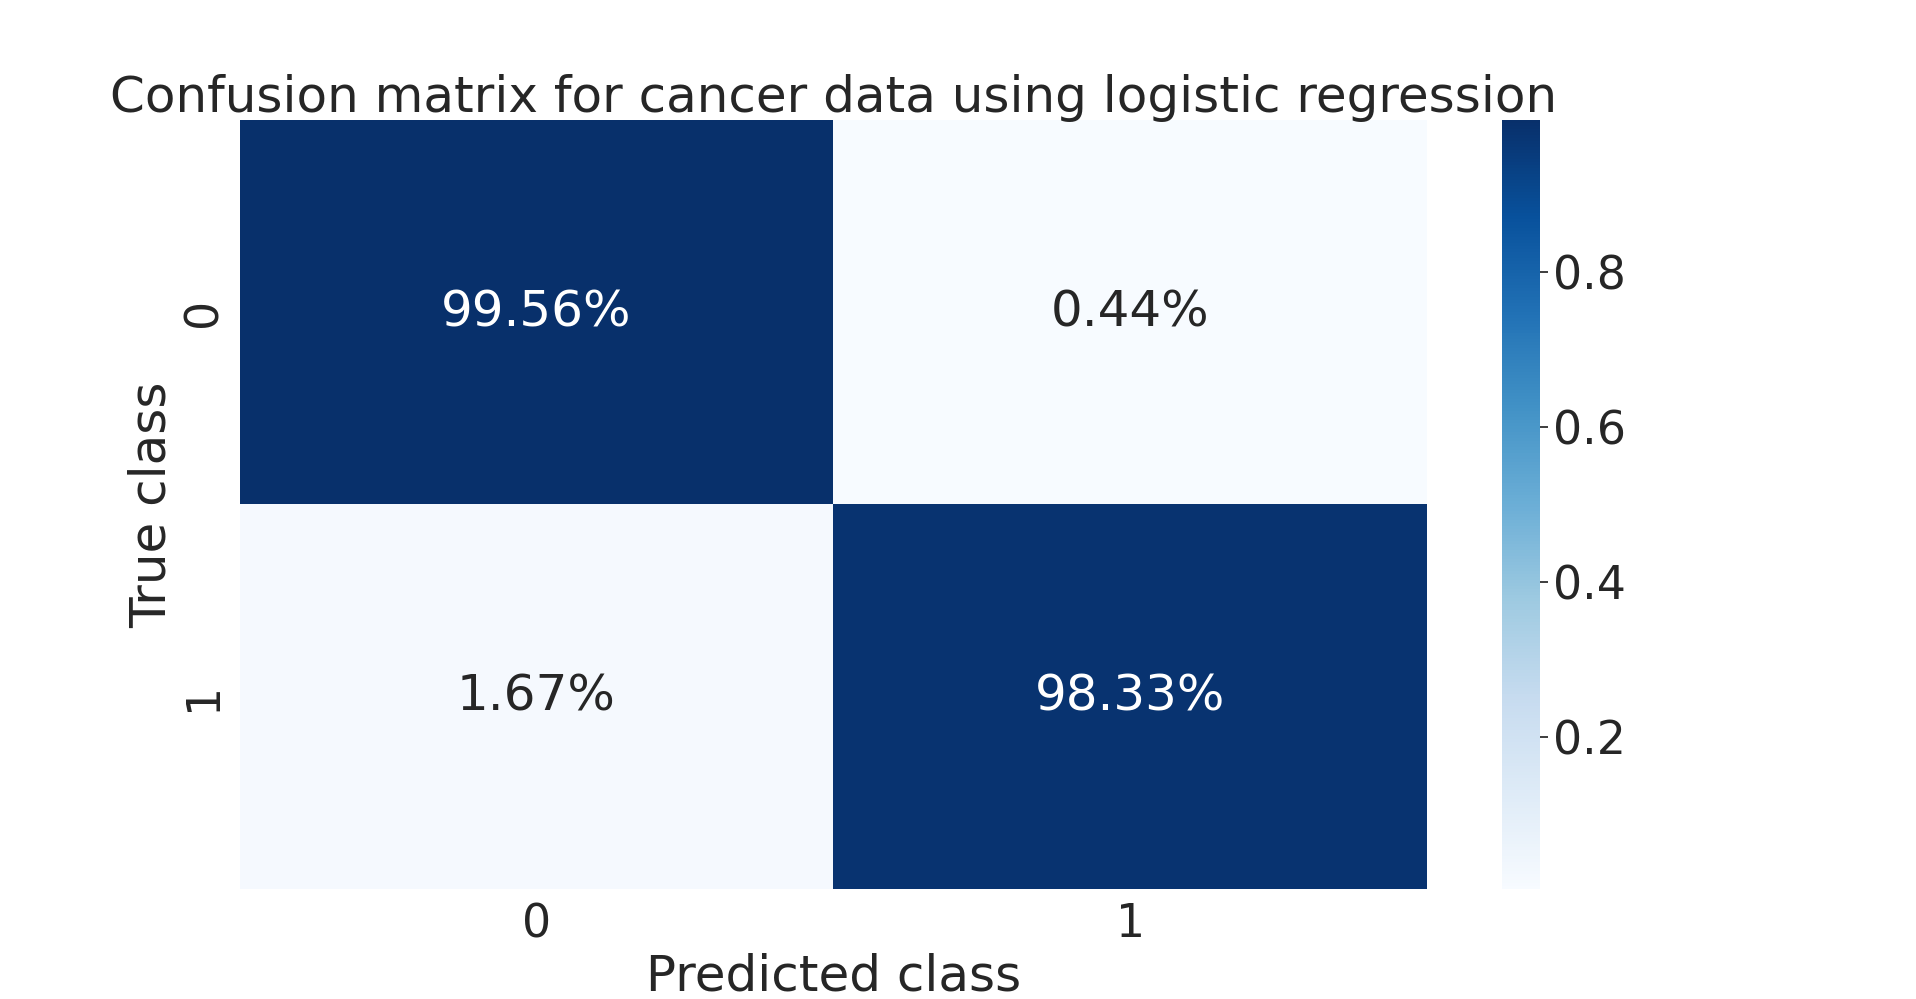
\includegraphics[width=5in]{figure/conf_mat_logreg_cancer.png}}
\caption{Confusion matrix for the cancer dataset using logistic regression}
\label{cancerconflog}
\end{figure}
\section{Conclusion}


In this paper we have studied supervised learning algorithms used for classification and regression problems, using the numerical optimization technique of gradient descent as a means of finding an optimal solution. We have observed how different schedulers improve the performance of our gradient descent, and found that amongst all the schedulers we tested, Adam and AdaGrad exhibited the best performance overall, achieving MSE's that were $32\%$ lower than the other schedulers in our testing. Using these schedulers, we solved regression and classification problems with our neural network implementation, but found that it underperformed compared to simpler models. For regression, our network achieved an MSE of $0.004781$, $24\%$ higher than a regular polynomial fit using the normal equations. In classification, our network achieved accuracies above $98\%$ for both the Wisconsin Breast Cancer and MNIST datasets, but regular logistic regression also achieved accuracies above $98\%$, in a much shorter time. To build upon the resarch conducted in this paper, one avenue to explore is to use larger and more complicated datasets, or to use different forms of neural networks such as convolutional neural networks.

\bibliographystyle{apalike}
\bibliography{bibliography}

\section*{Appendix A: Plots and tables}

The next pages contain plots and tables that are of interest.

\begin{table*}[h]
\caption{This table shows the file which created every plot in the report}
\begin{center}
\label{allparamstable}
\begin{tabular}{c | l l l}
Figure & Shell command \\
\hline
\ref{verification} & \texttt{python3 verification.py}\\
\ref{constant_v_momentum} & \texttt{python3 constant\_v\_momentum.py}\\
\ref{batch_constant_v_momentum} & \texttt{python3 constant\_v\_momentum.py}\\
\ref{heatmap} & \texttt{python3 task\_a.py}\\
\ref{adam_v_adagrad} & \texttt{python3 unknown.py}\\
\ref{msebymodelfranke} & \texttt{python3 bycomplexityfranke.py}\\
\ref{predterrain} & \texttt{python3 task\_b.py}\\
\ref{cancerarchcompsigmoid} & \texttt{python3 bycomplexitycancer.py}\\
\ref{cancerarchcomp} & \texttt{python3 bycomplexitycancer.py}\\
\ref{cancerconf} & \texttt{python3 task\_d.py}\\
\ref{cancerlogneur} & \texttt{python3 task\_d.py}\\
\ref{cancerconflog} & \texttt{python3 task\_d.py}\\
\ref{sgdbatch} & \texttt{python3 task\_a.py}\\
\hline
\end{tabular}
\end{center}
\end{table*}

\begin{figure}[H]
\centerline{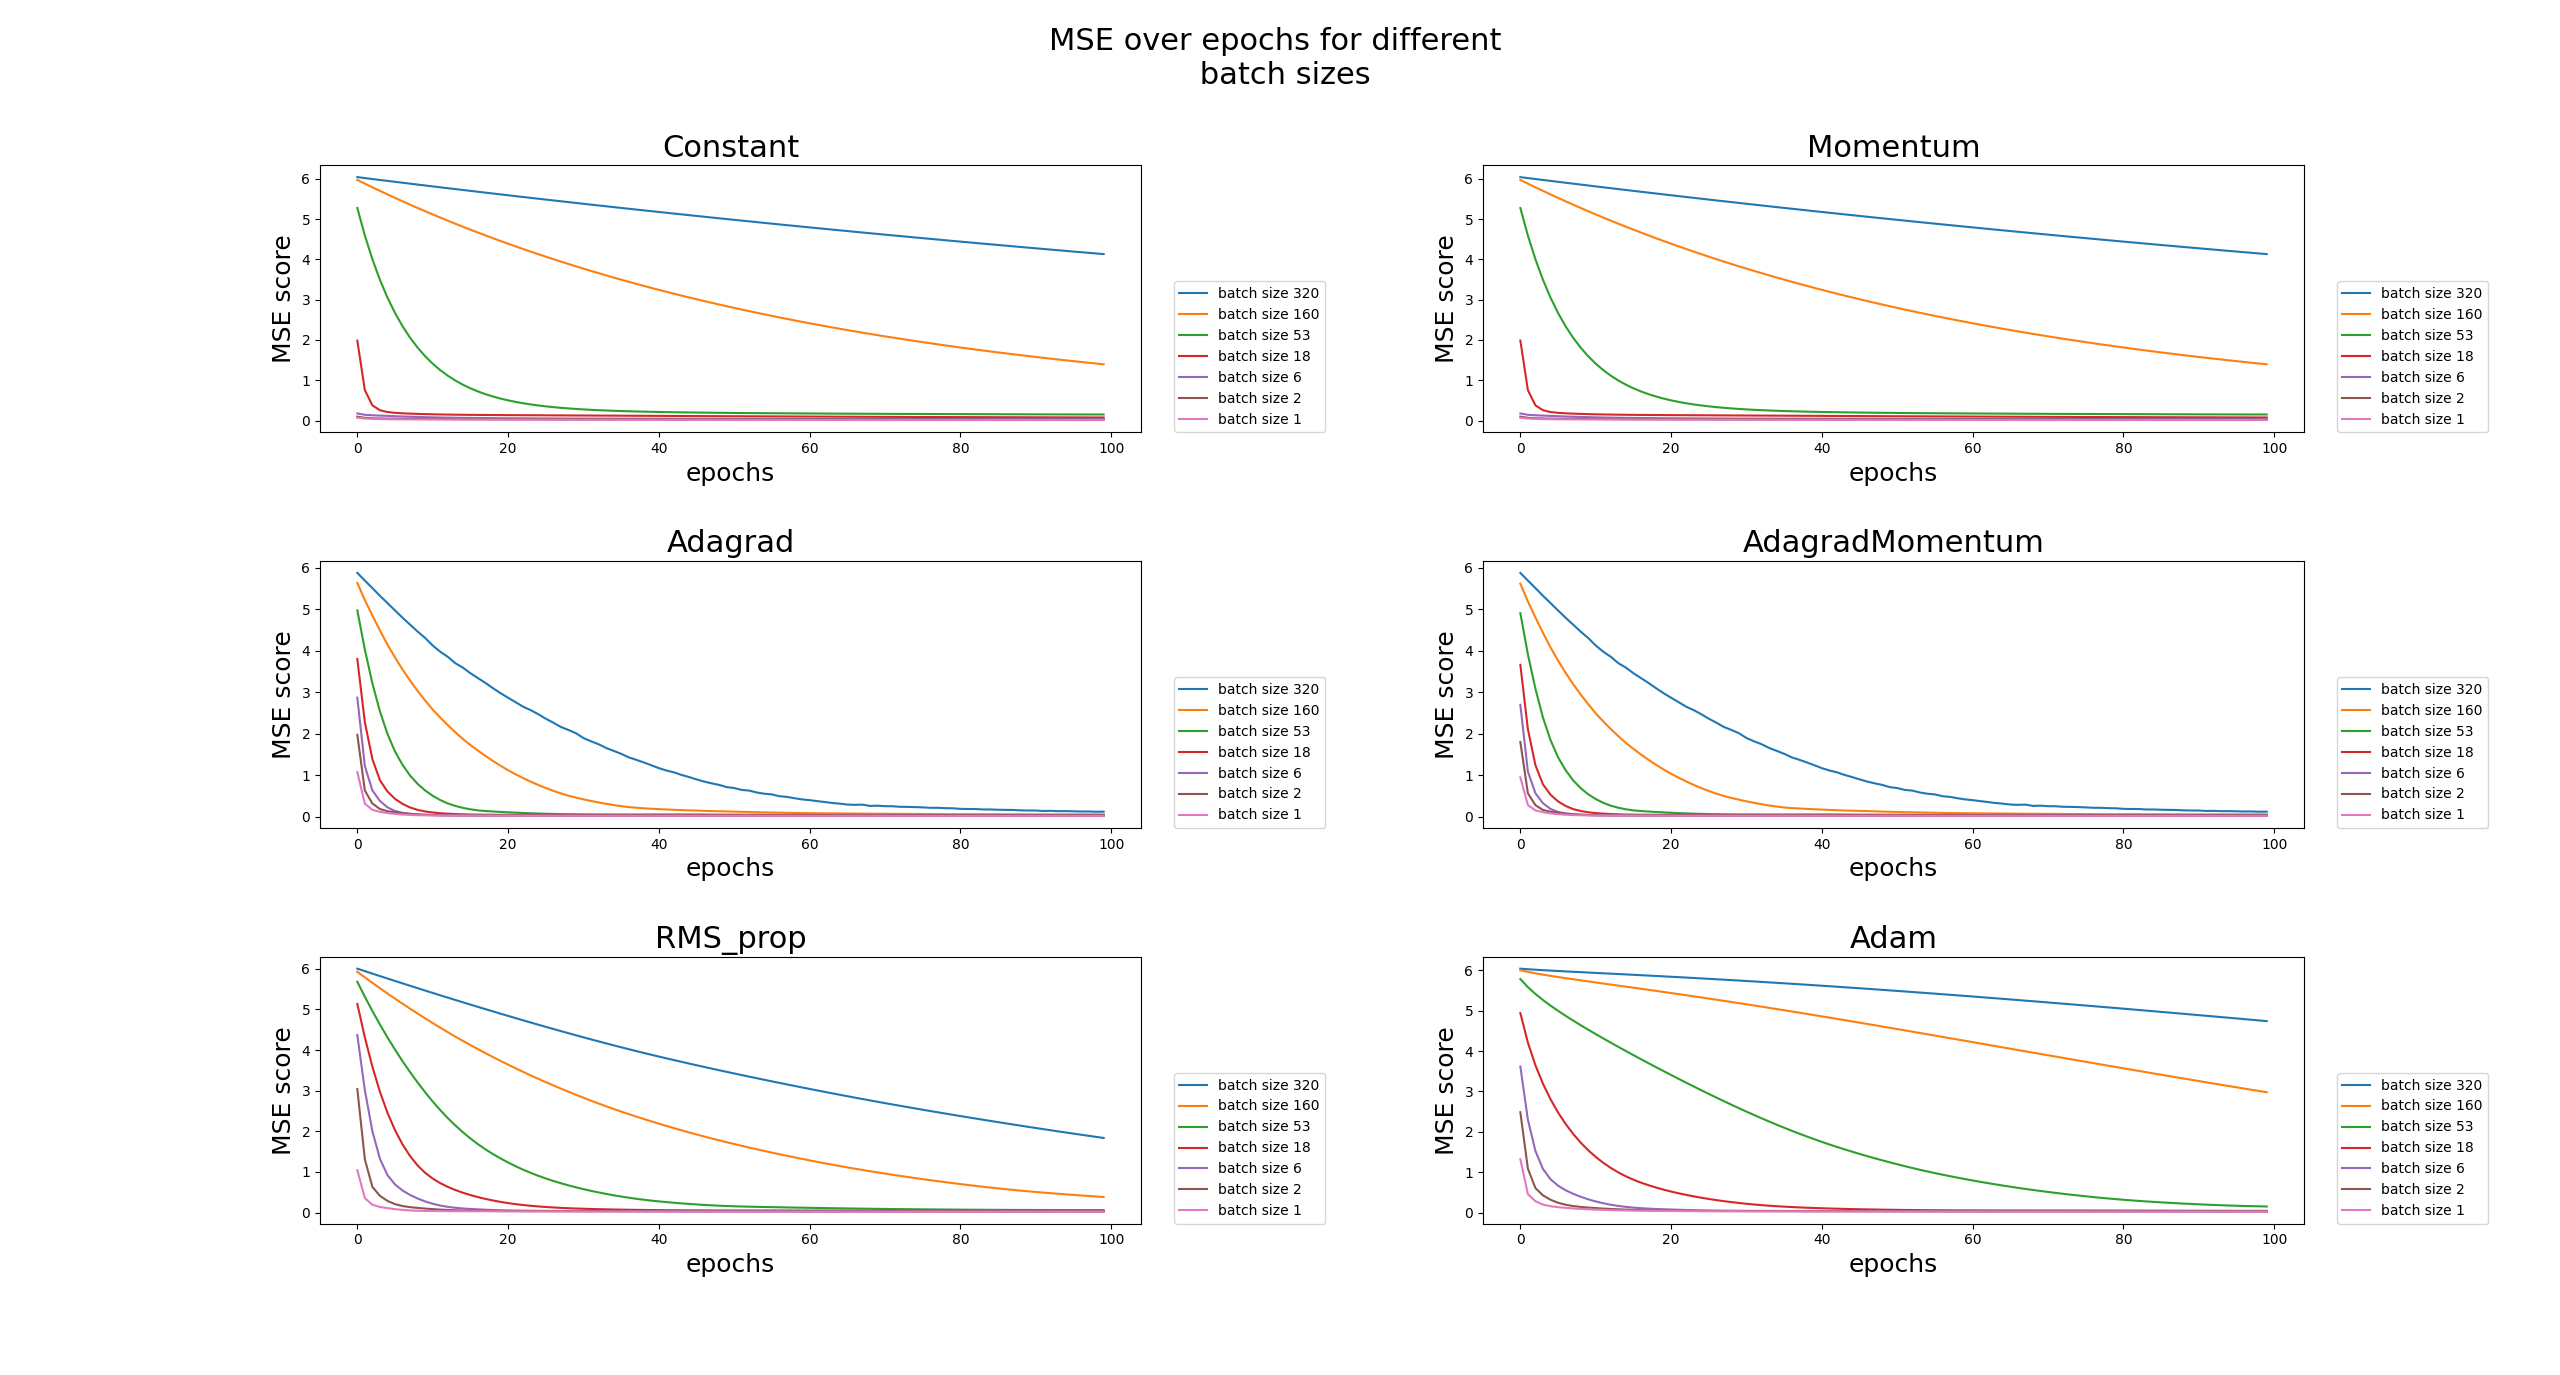
\includegraphics[width=7in]{figure/SGD_batch_size_100e.png}}
\caption{MSE over epochs for different batch sizes, for all different schedulers}
\label{sgdbatch}
\end{figure}

\begin{figure}[H]
\centerline{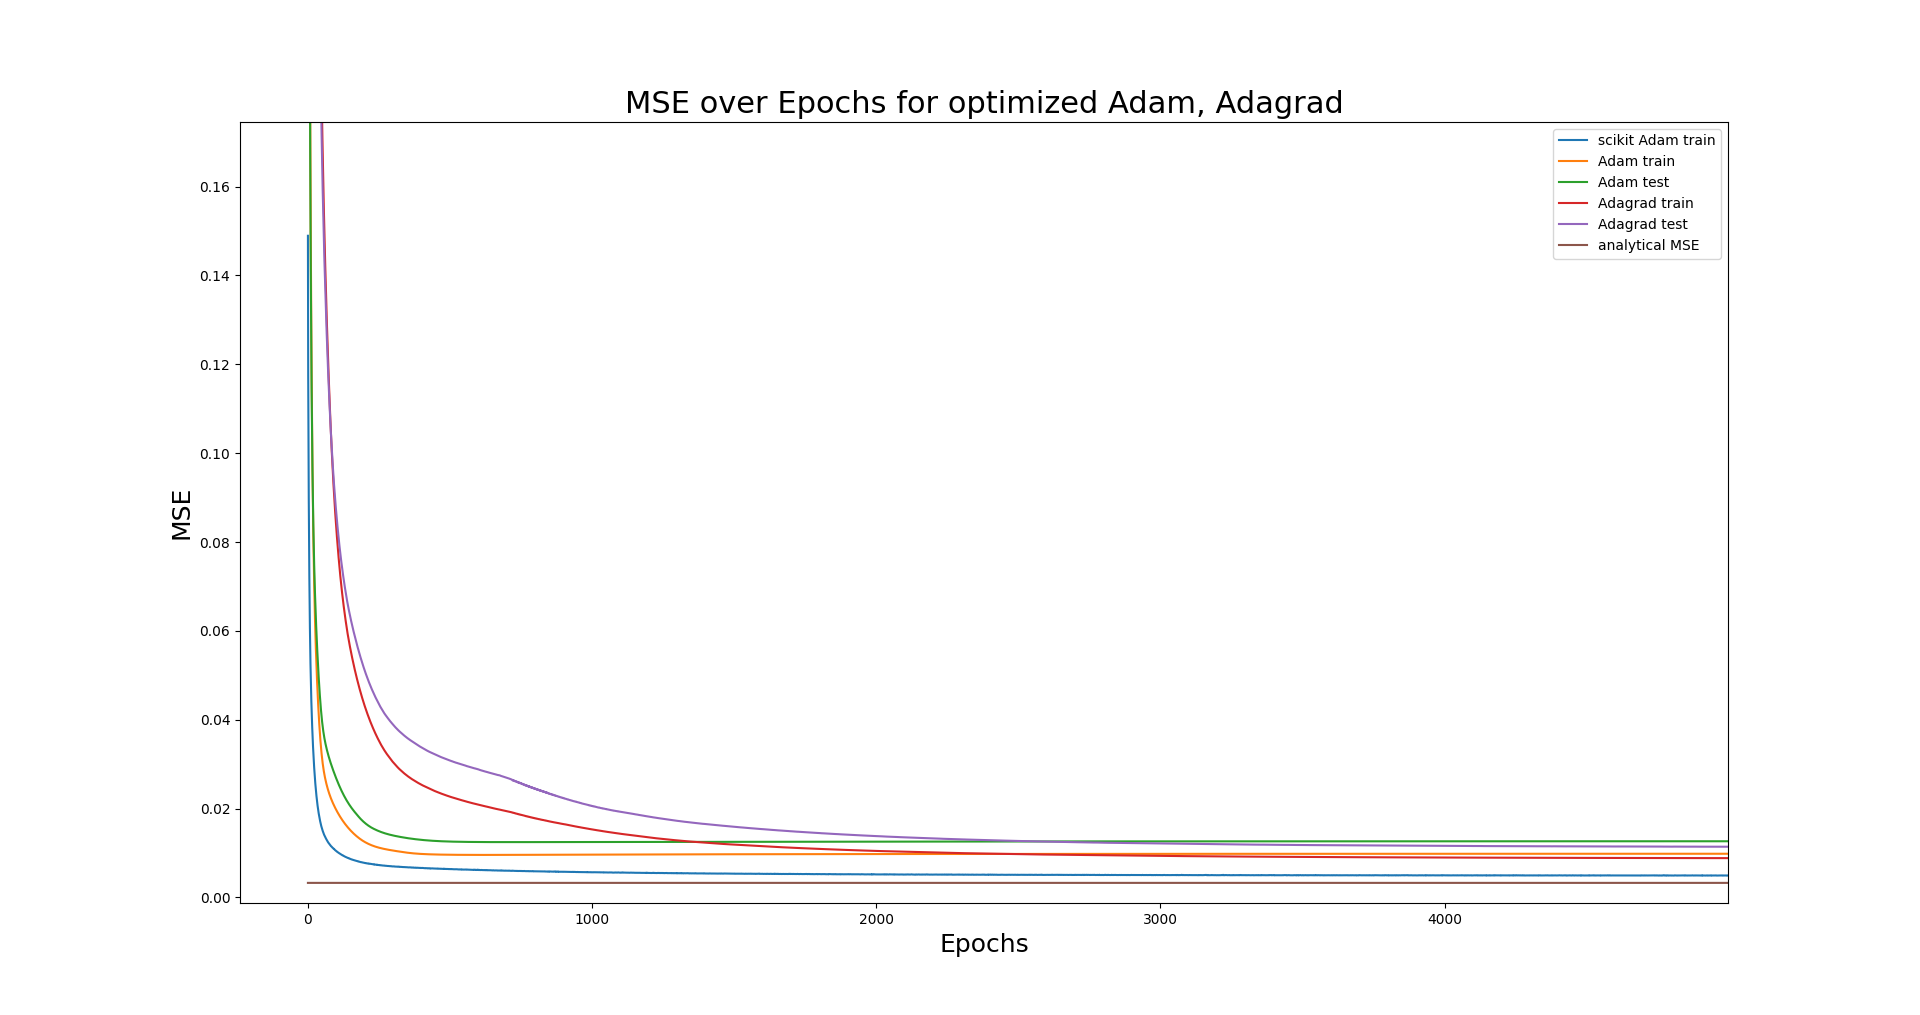
\includegraphics[width=7in]{figure/5000e_adam_v_adagrad.png}}
\caption{MSE test error over 5000 epochs for Adam and Adagrad schedulers}
\label{adam_v_adagrad}
\end{figure}

\end{document}
